\documentclass[11pt, a4paper]{article}

% --- UNIVERSAL PREAMBLE BLOCK ---
\usepackage[a4paper, top=2.5cm, bottom=2.5cm, left=2cm, right=2cm]{geometry}
\usepackage[english]{babel}

%%%% Standard Packages
\usepackage{graphicx}%
\usepackage{multirow}%
\usepackage{amsmath,amssymb,amsfonts}%
\usepackage{amsthm}%
\usepackage{mathrsfs}%
\usepackage[title]{appendix}%
\usepackage{xcolor}%
\usepackage{textcomp}%
\usepackage{booktabs}%
\usepackage{algorithm}%
\usepackage{placeins}
\usepackage{algpseudocode}
\usepackage{amsmath}
\usepackage{booktabs}
\usepackage{tabularx}
\usepackage{array}
\usepackage{algorithm}
\usepackage{algpseudocode}
\usepackage{setspace}
\usepackage{longtable}
\usepackage{amsmath}
\usepackage[hidelinks]{hyperref}
\usepackage{algpseudocode}%
\usepackage{float} % for [H]
%%%%

\usepackage{tikz}
\usetikzlibrary{arrows.meta, positioning, shapes.geometric}

\theoremstyle{plain}%
\newtheorem{theorem}{Theorem}%  meant for continuous numbers
\newtheorem{proposition}[theorem]{Proposition}% 

\theoremstyle{remark}%
\newtheorem{example}{Example}%
\newtheorem{remark}{Remark}%

\theoremstyle{definition}%
\newtheorem{definition}{Definition}%

\begin{document}

\title{\textbf{Structure-Aware and Gold-Summary-Guided Abstractive Summarization for Long Legal Judgments}}

\author{
    \textbf{Harshit Mahour}\textsuperscript{1}\thanks{harshitmahour360@gmail.com}, \ 
    \textbf{Amit Kumar Nandanwar}\textsuperscript{1}\thanks{its.abhishek.patel.org@gmail.com}, \ 
    \textbf{Abhishek Patel}\textsuperscript{1}\thanks{its.abhishek.patel.org@gmail.com} \\
    \vspace{0.2cm} \\
    \textsuperscript{1}Department of CS, IIIT Bhopal, Bhopal, India
}
\date{}

\maketitle

\begin{abstract}
Legal judgements are usually lengthy, detailed and hard to read rapidly because critical information is dispersed throughout facts, issues, arguments, reasoning and the final order. Consequently, automatic summarization in this context poses an inherently difficult problem, particularly with regard to the resulting summary’s conciseness and faithfulness . This paper presents CSS-LED, a structure-aware and salience-guided abstractive summarization framework for long legal judgments. The name CSS-LED denotes a Cluster-conditioned, Structure-aware, Salience-skeleton-guided Longformer Encoder-Decoder framework. The proposed method begins with cleansing the judgment text and segregating it into the corresponding legal sections and appending a semantics case level cluster token. It then builds a salience skeleton by selecting important source sentences that are closely related to the expert headnote. The cluster token, salience skeleton, and structured judgment are combined and given to a Longformer Encoder-Decoder model for summary generation. Experiments on the IN-ABS dataset show that CSS-LED produces more focused and better-structured legal summaries and outperforms extractive baselines and Plain LED.
\end{abstract}

\noindent\textbf{Keywords:} Legal judgment summarization, abstractive summarization, salience skeleton, structure-aware representation, Longformer Encoder-Decoder

\section{Introduction}

Court records are now being digitized on a large scale, and this has made many legal judgments available through online repositories. A legal judgment typically consists of separate parts of a case such as facts, legal issues, arguments of both sides, reasoning of the court, cited precedents and finally the final verdict. Because of this, legal judgments are a crucial resource for anyone whether you are lawyers, judges, researchers, litigants, and part of legal information systems. But their length and legalese make it harder to quickly identify the most relevant information. Due to this practical importance, automatic legal judgment summarization has become an important research area in legal NLP ~\cite{b1,b2}. However, legal judgments are typically very long, domain specific and written in complex legal language. This makes them harder to summarize than general documents, because the summary is mandatory to be short and readable, but also factually valid and legally relevant.  

Digging through an entire legal judgment takes time and patience. These documents are often long, densely worded and not exactly light reading unless you are very familiar with the law. So even experienced lawyers, researchers or anybody else find it hard to get what they really need.Previous legal summarization methods have addressed this problem using extractive and abstractive approaches ~\cite{b1,b2}. Some studies also look at legal judgments through rhetorical roles such as facts, issues, arguments, reasoning, and decisions ~\cite{b3}. However, these methods are still not sufficient for long legal judgments because recent abstractive models and large language models suffer from input-length restrictions, chunking issues, and factual inconsistency ~\cite{b4, b5}. Hence, there is a need for an effective automatic legal judgement summarisation method which can produce a short, clear and reliable summary without forcing the users to read the complete judgement.

Previous studies of legal judgement summarisation mainly used extractive methods to select important sentences from the judgement. These methods used sentence position, cue words, graph based ranking and rhetorical roles such as facts, issues, arguments, reasoning and decisions to identify legally useful content [2,3, 11,18]. Such methods are useful because they keep the original wording of the judgment and reduce the chance of changing the meaning. However, most of them still give long or repeated summaries, and they do not always produce a short headnote-like summary [1, 19].

Later, researchers also tried abstractive summarization models, so that the summaries could be shorter, clearer and easier to read. Models such as pointer-generator networks, BART, T5, PEGASUS, and legal-domain pretrained models have been studied for this task [4,7–10,12,13]. Recently, large language models have been used as well, as they can generate fluent text and follow instructions well [5,14–17]. Long-document transformer models such as Longformer, BigBird, and LongT5 further tried to handle the length of legal judgments by allowing larger input contexts [20–23].

The problem is not solved properly even after these methods. The legal judgments are too long and this is a major reason. A single judgment may contain facts in the starting part, then arguments in the middle portion, and after that the court's reasoning or final order is placed at near  the end. Therefore, shortening by truncation or chunking may cause missing some key legal points or losing the relationship between them [5, 6]. Abstractive models and LLMs may also generate fluent but unsupported content, omit important facts, or change the relation between issues and decisions [24, 25]. Another major limitation is the most existing methods can't make good use of the internal structure of legal judgments.Hence there is a need for a summarization method that can jointly utilize legal structure and important content signals, so that the summary generated is concise, coherent and factually reliable.

To tackle these challenges, this paper puts forward a structure-aware and salience-guided abstractive summarization framework for lengthy legal judgments. In the proposed work, the legal judgment is first cleaned by removing common noise such as repeated headers, page artifacts, broken text and other non-informative content. The judgment is arranged by its main case elements, moving from facts and issues to arguments, reasoning, and the final decision. That helps the model to understand how the case is aligned. The model looks at things, like facts and issues and arguments and reasons and the final decision to learn the underlying structure of the case [3]. Then, a salience skeleton is extracted from the judgement to highlight the legally important sentences and reduce loss of key information in long-document processing. Finally, the salience skeleton and structured judgment representation are given to a Longformer Encoder–Decoder model for generating a compact headnote-like summary [20, 21]. So the new method is supposed to make content selection better and also make use of legal discourse structure. Hence, capturing the main legal aspects and keeping in close relation to the decision, the summary does [24, 25].

The main contributions of the proposed work are:
\begin{itemize}
    \item A structure-aware legal summarization framework is suggested that captures the internal structure of legal rulings by representing them in segments, namely, facts, issues, arguments, reasoning, and final order.
    \item An approach is derived on the concept of salience skeleton extraction for identifying the significant parts of legal text, especially from lengthy judgments, in order to overcome information loss caused by truncation or chunking.
    \item An LED-based long-document generation framework is used with semantic cluster conditioning to generate compact abstractive legal summaries.
\end{itemize}

\section{Related Work}

Several approaches have been used to study legal judgment summarization, including: extractive sentence selection; neural based abstractive generation; transformer models for processing long documents; and more recent approaches using LLMs. This paper will discuss these approaches in detail. 
More specifically, we will examine them methodically, starting with the traditional extractive summary method and working our way up to pretrained abstractive models, long-document transformers, and prompt-based LLMs.
It should be mentioned that some drawbacks are still inherent in these approaches, notably poor use of legal structure and imperfect salience modeling. 


\subsection{Legal Case Judgment Summarization}

Traditionally, early summarization of legal case judgments relied heavily on an extractive method, where key sentences from the source judgment were picked to organize a summary. These systems used signals such as sentence position, cue phrases, rhetorical roles, graph-based ranking, TextRank, LexRank, and systems such as CaseSummarizer to estimate sentence importance [2, 3, 11, 18]. A general extractive scoring function can be written as:
\begin{equation}
\text{Score}(s_i) = \alpha P(s_i) + \beta C(s_i) + \gamma R(s_i) + \delta G(s_i),
\end{equation}

where \(P(s_i)\), \(C(s_i)\), \(R(s_i)\), and \(G(s_i)\) denote the position, cue-phrase, rhetorical-role, and graph-ranking scores for sentence \(s_i\), respectively.

These techniques preserve original terminology and reduce the risk of hallucinations because they primarily replicate sentences from the judicial decision. However, the resulting summaries are often lengthy, repetitive, and only loosely coherent. While extractive methods preserve factual accuracy, they do not synthesize legal reasoning into a concise and well-structured summary in the manner of a legal expert [6,1].


\subsection{Legal Summarization Datasets and Benchmarks}

Research on legal summarization has constantly progressed in large numbers with the development of domain-specific datasets and benchmarks. Researchers have a genuine opportunity to evaluate summarizing techniques on real legal documents with collections such as CaseSummarizer [2], IN-ABS [11], CivilSum, MultiLexSum [28], LexSumm and LexAbSumm [26, 27], and EUR-Lex-Sum [29]. Legal judgements include a collection of discourses-facts, legal questions, lawyers arguments of both parties, arguments from the court, citations of court decisions in prior cases etc. And finally, conclusion. Hence, it is very difficult to summarize legal texts and a totally different kind of task. Evaluations have to match the level of complexity that you find in this domain.” Even with the presence of those benchmarks and its clear measurable settings, current systems still have a lot to improve in terms of how to deal with long judgments and take advantage of the internal structure of the legal documents further.

\subsection{Neural Abstractive Summarization}
The essence of neural abstractive summarization is using a model to generate a novel summary with a higher compression and a more human-like readability, rather than choosing an extractive process where the generated summary consists of source sentences. The first series of neural abstractive summarization models relied on the sequence to sequence frameworks with attention and further extended by the pointer-generator networks which generate word by word, copying the word with higher possibility and then generating the word. This enabled it to carry over words from the source language, though it did paraphrase them somewhat [7]. Models like BERTSum, BART [8], PEGASUS [10] and T5 [9] were used for abstractive summarization which improved the performance on the summarization task by better language understanding from large-scale corpora. Models for legal abstractive summarization like Legal-Pegasus and Legal-LED have also been developed for legal text and long judgments [10, 11, 21]. In general, abstractive summarization can be denoted as:

\begin{equation}
\hat{Y} = \arg\max_{Y} P(Y \mid X)
\end{equation}

where \(X\) is the source judgment and \(\hat{Y}\) is the generated summary.The summarization models are shorter and more readable than those extractive ones. Nevertheless, legal judgments have factual description, legal problems, arguments, reasoning, and the concluding decision in order, it is difficult for abstractive generation in a direct way. Abstractive models may skip crucial details, show wrong reasoning or create false claims. Hence, it gains readability at the sacrifice of factual correctness and content coverage in legal text.


\subsection{Long-Document Summarization}

Legal rulings can be considerably longer than the standard length limitations in Transformer models. Given that self-attention calculates all pairs interactions between tokens, complexity becomes quadratic in sequence length and so it's prohibitively expensive to process long documents:

\begin{equation}
O(L^{2})
\end{equation}

where (L) denotes the input sequence length. To avoid this problem most summarization systems employ either truncation or chunking techniques. It often happens however that essential legal information is spread over the length of a judgment, so that the facts of a case occur early on, arguments and legal reasoning mid-way, and decisions at the end. In this case it is easy for such methods to lose chunks of relevant information.
Several long-document architectures have been developed to overcome this problem. Longformer utilized local windows and global tokens in a sparse attention mechanism and LED applies it to summarization within an encoder--decoder setting [21]. BigBird use block-sparse patterns in their attention for scalability [22] and LongT5 adopts text-to-text pre-training to handle longer sequences through the usage of efficient attention [23]. Even though this effectively solves truncation and makes it possible for long documents to be processed, longer context alone does not tell the model which legal facts and reasoning should be most important and hence long-context models still need a specific salient guidance mechanism. 

\subsection{Large Language Models for Legal Summarization}

Recently, LLMs gain more attention due to their remarkable language generation and instruction following capabilities on summarization. For instance, GPT based models are capable of generating fluent, coherent and human-like summaries without task specific fine-tuning [14, 15, 17]. Such characteristics lead researchers to investigate the potential of applying LLMs to summarizing legal judgment where abstraction and natural language generation are critical. A legal ruling can potentially include a body of information which greatly exceeds the scope for LLMs. For processing the long documents, standard techniques usually apply chunking, sliding window, repetitive prompting or post-processing[11, 18]. This way the legal narrative will be separated and the connection between facts, arguments, judicial reasonings, and orders will be attenuated. Key facts omitted and inconsistency will arise in the generated summary. Hence, LLMs do provide a flexible structure but fail to perform the summary for scalable and faith worthy legal judgment summarization.


\subsection{Faithfulness and Evaluation Metrics}
The quality of the legal summaries should be assessed properly. Legal summaries are to be easily understandable and factual to the court decision. Any slight alteration in the part, statute, fact, issue, reasoning, or holding, will change the meaning of the decision legally. ROUGE, METEOR, and BERTScore are the commonly used metrics for automatic summarization quality evaluation. ROUGE is the most popular as there are already well-established metrics for estimating the overlap between machine and human summaries. N-gram overlaps measure the recall for word sequences and for pairs of sentences; Longest Common Subsequence measures summarization at the sentence level, and can compensate for reordered sentences. ROUGE is used for evaluating our proposed methods in this paper as well. However ROUGE has limitations. It only measures word overlap and so it can't approximate to what extent the legal meaning is accurately expressed or the information in the summary is factually correct. Lexical overlap as well as factual faithfulness should be taken into consideration for legal summaries.

\subsection{Positioning of Our Work}

Two major drawbacks of legal judgment summarization research (from above literature) are analyzed. Firstly, existing approaches could barely take care of global salience of documents, so if a judgment document is lengthy, important facts, issues, arguments, reasoning, and the final order might be missed out. Secondly, legal text has already embedded some structural features, like facts, issues, arguments, reasoning and final order, but these approaches cannot leverage these structures sufficiently. Based on these shortcomings, this work presents a structure-aware and gold-summary-guided abstractive summarization pipeline. The developed pipeline first processes the legal judgment to be segmented into legal sections. After that a salience skeleton is generated guided by the gold summary to mark salient sentences.   Finally, the cluster token, salience skeleton, and structured document are combined as:

\begin{equation}
X_{\text{input}} = T_{\text{cluster}} \oplus B_{\text{skel}} \oplus B_{\text{doc}}
\end{equation}

and these key segments are fed to the long-document generator, implemented in an LED model. Therefore, our framework achieves extractive salience selection and abstractive long document generation with structure flow in legal judgments.

\section{Proposed Methodology}
\label{sec:methodology}

In this section we present the proposed methodology of legal judgment summarization . An developed system takes as input a legal judgment and provides as output an abstractive summary of the input legal judgment. The legal judgment is first cleaned, structurized, converted into salience-guided representation and then passed to Longformer Encoder-Decoder model for summary generation rather than passing the entire judgment directly to the model ~\cite{b21}.
Let the dataset be represented as:

\begin{equation}
\mathcal{D}=\{(X_i,Y_i)\}_{i=1}^{N}
\end{equation}

where \(X_i\) denotes the \(i^{\text{th}}\) legal judgment, \(Y_i\) denotes its corresponding gold summary, and \(N\) is the total number of judgment-summary pairs. The overall objective of the proposed model is to learn a mapping function:

\begin{equation}
F: X_i \rightarrow \hat{Y}_i
\end{equation}

where \(\hat{Y}_i\) is the generated summary. In the proposed framework, this mapping is performed through a structured input representation:

\begin{equation}
\hat{Y}_i = \mathrm{LED}(X_i^{\text{input}})
\end{equation}

The final input sequence is constructed as:

\begin{equation}
X_i^{\text{input}} =
T_{\text{cluster}} \oplus B_{\text{skel}} \oplus B_{\text{doc}}
\end{equation}

where \(T_{\text{cluster}}\) is the semantic cluster token, \(B_{\text{skel}}\) is the salience skeleton, \(B_{\text{doc}}\) is the structure-aware document block, and \(\oplus\) denotes concatenation. The complete flow of the proposed CSS-LED framework is summarized in Algorithm~1.

now fix this i want 30 steps 

\begin{algorithm}[H]
\caption{Mathematical Procedure of the Proposed CSS-LED Model}
\label{alg:proposed_algorithm}
\begin{algorithmic}[1]
\Require Dataset $\mathcal{D} = \{(X_i, Y_i)\}_{i=1}^{N}$, Number of clusters $K$, Similarity threshold $\tau$
\Ensure Generated summary $\hat{Y}_i$ and Evaluation Metrics
\For{each matched pair $(X_i, Y_i) \in \mathcal{D}$}
    \vspace{2pt}
    \State \textbf{Phase 1: Context Conditioning}
    \State $\mathbf{z}_i \gets \phi(X_i)$ \Comment{Extract dense semantic sentence embeddings}
    \State $c_i \gets \text{K-Means}(\mathbf{z}_i, K)$ \Comment{Assign to semantic cluster $c_i \in \{1 \dots K\}$}
    \State $T_{\text{cluster}} \gets \langle CL_{c_i} \rangle$ \Comment{Generate semantic cluster token}
    \vspace{2pt}

    \State \textbf{Phase 2: Structure-Aware Segmentation}
    \State $X'_i \gets (f_{\text{boiler}} \circ f_{\text{punct}} \circ f_{\text{space}})(X_i)$ \Comment{Domain-specific noise removal}
    \State $B_{\text{doc}} \gets \text{Segment}(X'_i)$ \Comment{Map to canonical sections $\mathcal{S}$}
    \vspace{2pt}

    \State \textbf{Phase 3: Salience Skeleton Extraction}
    \State $S \gets \{s_1, s_2, \dots, s_M\} \in X'_i$ \Comment{Source judgment sentences}
    \State $T \gets \{t_1, t_2, \dots, t_N\} \in Y_i$ \Comment{Gold summary sentences}
    \State Calculate $\mathbf{M}_{n,m} = \frac{\mathbf{v}(t_n) \cdot \mathbf{v}(s_m)}{\|\mathbf{v}(t_n)\| \, \|\mathbf{v}(s_m)\|}$ \Comment{TF-IDF cosine similarity matrix}
    \State $Score(s_m) \gets \max_{1 \leq n \leq N} \mathbf{M}_{n,m}$
    \State $B_{\text{skel}} \gets \text{Sort}_{original}(\{s_m \mid Score(s_m) \geq \tau\})$ \Comment{Extract ordered skeleton}
    \vspace{2pt}

    \State \textbf{Phase 4: Abstractive Generation}
    \State $X_{\text{input}} \gets T_{\text{cluster}} \oplus B_{\text{skel}} \oplus B_{\text{doc}}$ \Comment{Formulate hybrid sequence input}
    \State $\hat{Y}_i \gets \text{LED}(X_{\text{input}})$ \Comment{Autoregressive decoding via sparse attention}
\EndFor

\State Evaluate $\hat{Y}_i$ using Rouge-1, R-2, and R-L P, R, F-1 scores.
\Comment{Summary quality evaluation}
\end{algorithmic}
\end{algorithm}


This approach, in mathematical terms, integrates semantic case conditioning, structure-aware legal representation, salient skeleton extraction and LED-based abstractive generation for long legal judgment summarization.

The overall system architecture that we propose can be seen as a multi-stage pipeline (in Fig.~\ref{fig1}). This involves: dataset preparation, semantic case conditioning, pre-processing, structure aware segmentation, salient skeleton extraction and abstractive summary generation through LED.


\begin{figure}[H]
\centering
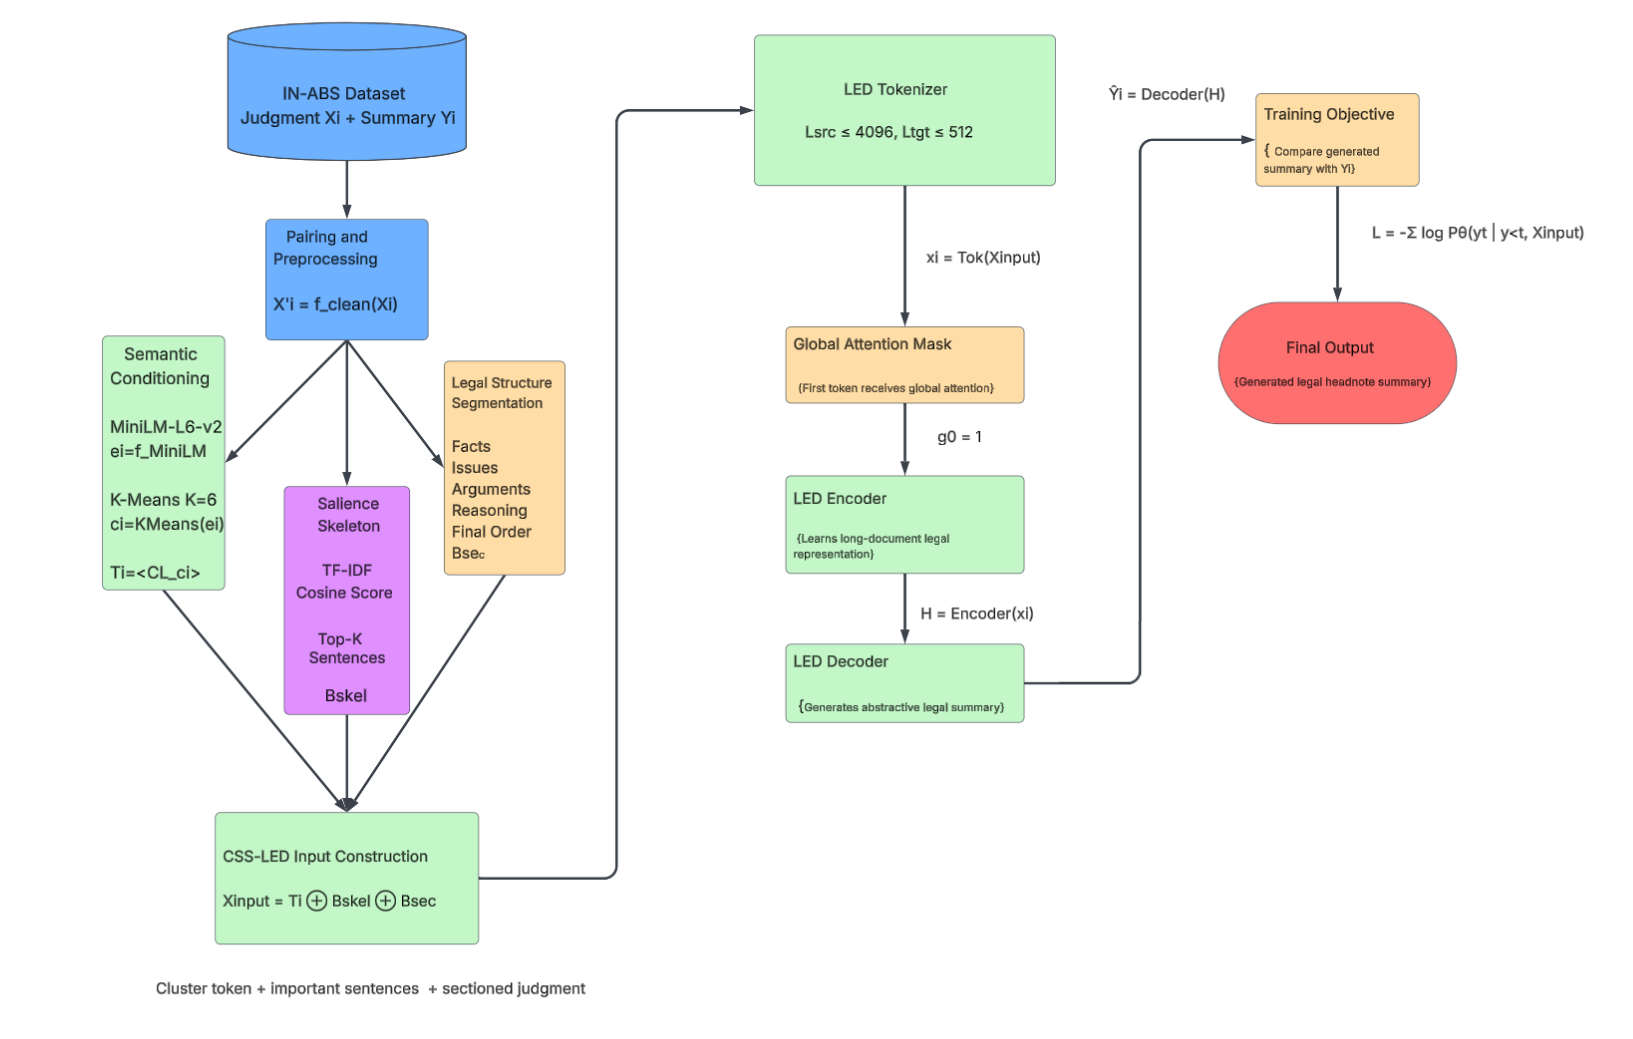
\includegraphics[width=0.9\textwidth]{FA.png}
\caption{\textbf{Proposed architecture for structure-aware legal judgment summarization.}}
\label{fig1}
\vspace{-2mm}
\end{figure}

\subsection{Dataset Preparation} 

In this paper, we use the IN-ABS dataset for the task of legal judgment summarization ~\cite{b1}. Each data point of the dataset consists of a legal judgment document, and a summary written by human annotators. The entire data set can be formally written as: 

\begin{equation}
\mathcal{D}=\{(X_i,Y_i)\}_{i=1}^{N}
\end{equation}

where \(X_i\) denotes the \(i^{\text{th}}\) legal judgment, \(Y_i\) denotes its gold summary, and \(N\) is the total number of matched judgment-summary pairs.

In the implementation, a pair of judgment and summary is chosen only when the judgment file as well as the summary file is present.The valid dataset can, therefore, be written as:

\begin{equation}
\mathcal{D}_{\text{valid}}=
\{(X_i,Y_i)\mid X_i \neq \emptyset \ \text{and} \ Y_i \neq \emptyset\}
\end{equation}

For computational feasibility, the training data are capped to 6000 cases:

\begin{equation}
N_{\text{cap}}=6000
\end{equation}

From this capped training set, 10\% of the samples are used for validation:

\begin{equation}
N_{\text{val}}=0.10 \times N_{\text{cap}}
\end{equation}

\begin{equation}
N_{\text{val}}=0.10 \times 6000=600
\end{equation}

The remaining samples are used for model fine-tuning:

\begin{equation}
N_{\text{train}}=N_{\text{cap}}-N_{\text{val}}
\end{equation}

\begin{equation}
N_{\text{train}}=6000-600=5400
\end{equation}

Hence, a total of 5400 training, 600 validation, and test samples of the available IN-ABS test set are in the final experimental split. The created pairs, index file containing case ID, split type, path to judgment and path to summary is used in following steps. This index is further used in subsequent stages to extract preprocess, structure-aware segmentation, salience skeleton, and LED training.

\subsection{Semantic Case Conditioning}

The legal judgments may be divided into various semantic types such as criminal, civil, constitutional, service related and tax cases. If all the cases are processed similarly then this case level context may not be captured by the model. Hence a weak semantic signal is added prior to the generation of summary.

A dense document embedding is produced for each of the cleaned judgments \(X'_i\) using the sentence transformer model MiniLM ~\cite{b41}. The process of embedding can be visualized as follows:

\begin{equation}
z_i=\phi(X'_i)
\end{equation}

where \(\phi(\cdot)\) denotes the sentence-transformer embedding function and \(z_i \in \mathbb{R}^{d}\) is the dense representation of the \(i^{\text{th}}\) judgment.

Once embeddings for all judgments have been produced K-Means clustering can be used to group semantically similar cases together. For the case of using: The number of cluster to be used in this scenario is set as:

\begin{equation}
K=6
\end{equation}

In each legal judgment, it is transformed to the dense semantic embedding via the MiniLM model. It is clustered via K-Means to get a case level semantic cluster as the shows in Figure~\ref{fig:minilm_semantic_clustering}

\begin{figure}[H]
\centering
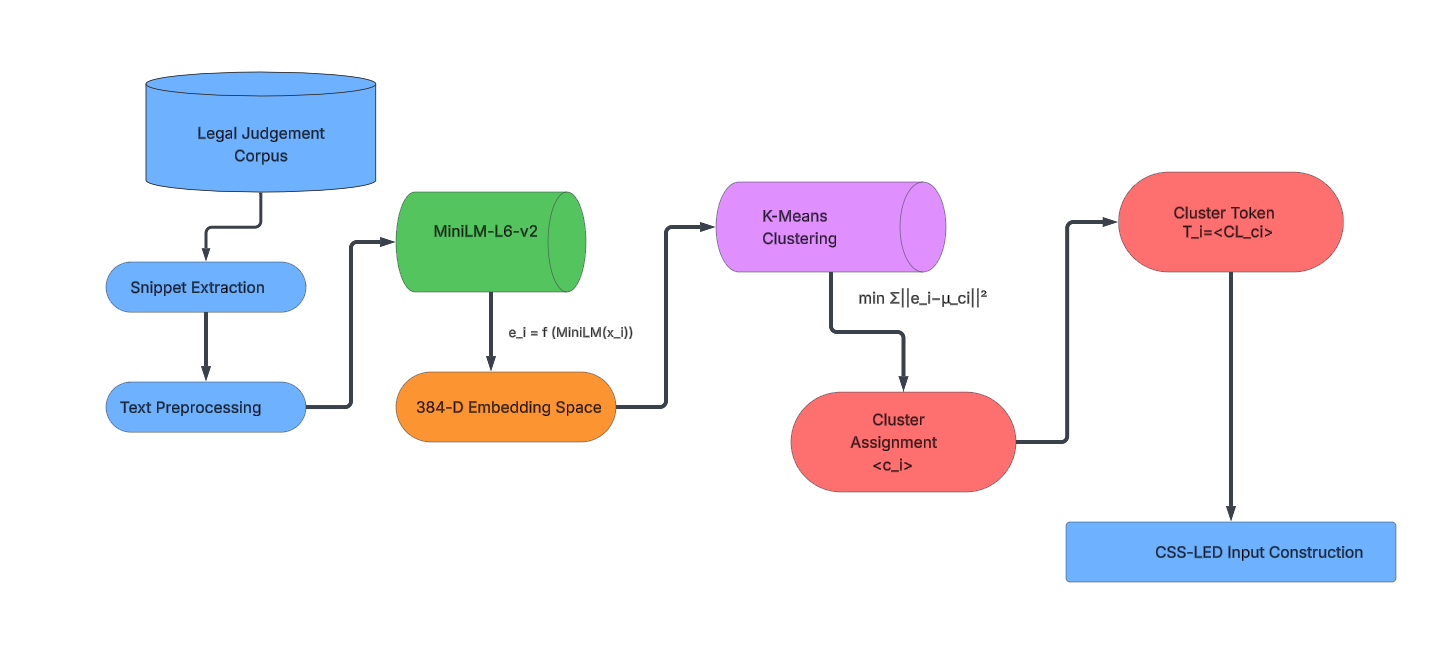
\includegraphics[width=0.9\textwidth]{Bert.png}
\caption{\textbf{MiniLM-based semantic embedding and clustering process used for case-level context conditioning.}}
\label{fig:minilm_semantic_clustering}
\vspace{-2mm}
\end{figure}

The chosen cluster ID is then transformed into a special token, for example, ($\langle $\mathrm{CL}_2$ \rangle$), and prepended to the overall model input.


The clustering objective is defined as:

\begin{equation}
\arg\min_{C}\sum_{k=1}^{K}\sum_{z_i\in C_k}
\|z_i-\mu_k\|^2
\end{equation}

where \(C_k\) denotes the \(k^{\text{th}}\) cluster and \(\mu_k\) is its centroid. Each judgment is assigned a cluster id \(c_i\) as:

\begin{equation}
c_i=\arg\min_{k}\|z_i-\mu_k\|^2
\end{equation}

The assigned cluster id is then converted into a special cluster token:

\begin{equation}
T_{\text{cluster}}=\langle CL_{c_i}\rangle
\end{equation}

For example, if a judgment is assigned to cluster 2, its cluster token becomes:

\begin{equation}
T_{\text{cluster}}=\langle CL_2\rangle
\end{equation}

This token is later added at the beginning of the model input:

\begin{equation}
X_i^{\text{input}}=
T_{\text{cluster}}\oplus B_{\text{skel}}\oplus B_{\text{doc}}
\end{equation}

where \(B_{\text{skel}}\) is the salience skeleton, \(B_{\text{doc}}\) is the structured document block, and \(\oplus\) denotes concatenation. Therefore, the model receives a simple case-level semantic signal before generating the final summary.

\subsection{Domain-Specific Preprocessing}

Raw decisions cannot be summarized so easily, however, because the amount of un-substantive material is very large. A judgment may include headings, page numbers, reportable or non-reportable indications, duplicated case numbers, judge signatures, date lines, locations, split sentences, gaps, etc. All of these elements are of use in the format of the original judgment, but do not directly contribute to its legal significance ~\cite{b1,b4}.

If we pass such noisy text into the summarization model directly, it will take up valuable input space and make the model pay less attention to the legally relevant contents. Because legal judgments are typically very long already, filtering out the noise before the structure-aware segmentation and LED-based generation is critical. The model hence transforms the raw judgement into a cleaner and more comprehensible form. 

Let the raw legal judgment be represented as \(X_i\). The cleaned judgment is denoted as:

\begin{equation}
X'_i=C(X_i)
\end{equation}

where \(C(\cdot)\) is the complete cleaning function. In the proposed system, this function is applied through three main operations:

\begin{equation}
X'_i=
(f_{\text{boiler}} \circ f_{\text{punct}} \circ f_{\text{space}})(X_i)
\end{equation}

Here, \(f_{\text{space}}\) handles spacing and line-break problems, \(f_{\text{punct}}\) normalizes punctuation and symbols, and \(f_{\text{boiler}}\) removes repeated legal boilerplate text. The same process can also be written step by step as:

\begin{equation}
X_i^{\text{space}}=f_{\text{space}}(X_i)
\end{equation}

\begin{equation}
X_i^{\text{punct}}=f_{\text{punct}}(X_i^{\text{space}})
\end{equation}

\begin{equation}
X'_i=f_{\text{boiler}}(X_i^{\text{punct}})
\end{equation}

Here $f{\text{space}}$ trims the redundant white spaces, $f{\text{punct}}$ standardizes the punctuation marks, and $f{\text{boiler}}$ trims the non-informative legal boiler plates. The main preprocessing rules are given in Table~\ref{tab:cleaning_rules}.

\begin{table}[H]
\centering
\caption{Heuristic rules used for legal document preprocessing.}
\label{tab:cleaning_rules}
\renewcommand{\arraystretch}{1.25}
\setlength{\tabcolsep}{4pt}
\begin{tabularx}{\linewidth}{@{}p{0.25\linewidth}X p{0.18\linewidth}@{}}
\toprule
\textbf{Noise Type} & \textbf{Examples} & \textbf{Action} \\
\midrule
Court metadata & Supreme Court of India, High Court, Reportable, Non-reportable & Removed \\
Case identifiers & Civil Appeal No., Criminal Appeal No., SLP, Petition No. & Removed if repeated \\
Pagination & Page numbers, page headers, page footers & Removed \\
Formatting noise & Extra spaces, broken lines, repeated symbols & Normalized \\
Administrative text & Location, registry text, judge signature blocks & Removed where non-substantive \\
\bottomrule
\end{tabularx}
\end{table}

Through this preprocessing step, non-substantive legal clutter is reduced, and the model is permitted to concentrate on the relevant legal content like facts, contentions, rationale and the ruling.

The first operation, \(f_{space}\), handles spacing-related noise in the judgment. It removes extra spaces, repeated new lines, tab spaces, and broken line characters, so that the text becomes more continuous before being passed to the tokenizer. The second operation, \(f_{punct}\), normalizes quotation marks, dashes, punctuation symbols, and invisible characters into a common format. This helps reduce unnecessary formatting differences in the text. The third operation, \(f_{boiler}\), removes redundant or non-informative legal patterns, such as court headings, appeal numbers, page numbers, reportable labels, judge signatures, and location or date information.
\\
In simple terms, the preprocessing stage applies the following rules:
\begin{enumerate}
\item Remove repeated court headings such as ``Supreme Court of India'' and High Court headings.
\item Remove labels such as ``Reportable'' and ``Non-Reportable'' because they do not add summary content.

\item Remove repeated case identifiers such as Civil Appeal No., Criminal Appeal No., SLP, and Petition No., if they appear as repeated metadata.

\item Remove page numbers, page headers, and page footers.

\item Remove judge signature blocks, location lines, and date lines when they are not part of the legal reasoning.

\item Normalize extra spaces, broken lines, punctuation marks, quotation marks, and special symbols.

\item Convert the cleaned text into a continuous readable form for further processing.

\end{enumerate}

Following the processing stages, X'i is essentially the significant legal text with few irrelevant items such as pre-processing information and cleaning errors. The format of the given text is largely composed of facts, issue, arguments, reasons and order. It is neither a summary and nor an extract. The cleaned judgment text is then fed to the subsequent stages for segmentation of the legal section, extraction of salience skeleton, and final abstractive summary generation.

\subsection{Structure-Aware Document Segmentation}

This output text consists mainly of fact, issue, arguments, reasoning and order. Once the cleanup is finished, the judgment can then be fitted into a template format of the formal part of a document. This is important because a judgment is not just a document; the implicit structure often follows a legal flow. First, the facts of the case are introduced, then the legal question or issues are addressed, followed by the arguments, judicial reasoning, and final order. Otherwise, the model may give equal weight to all sentences and fail to capture the actual contribution of each sentence to the judgment ~\cite{b3}.

The processed judgment is represented as \(X'_i\). 
The framework then classifies \(X'_i\) into five standard legal sections:

\begin{equation}
S = \{\text{FACTS}, \text{ISSUES}, \text{ARGUMENTS}, \text{REASONING}, \text{FINAL\_ORDER}\}
\end{equation}

Thus, the section-wise representation of the judgment can be written as:

\begin{equation}
X_i^{\text{sec}} =
\{X_i^{\text{facts}}, X_i^{\text{issues}}, X_i^{\text{args}}, X_i^{\text{reason}}, X_i^{\text{order}}\}
\end{equation}

Here, \(X_i^{\text{facts}}\) represents the factual background of the case, 
\(X_i^{\text{issues}}\) contains the main legal questions, \(X_i^{\text{args}}\) includes the 
arguments or submissions made by the parties, \(X_i^{\text{reason}}\) captures the 
reasoning given by the court, and \(X_i^{\text{order}}\) represents the final decision or order of the judgment.

The purpose of each legal section is summarized in Table~\ref{tab:section_schema}.

\begin{table}[H]
\centering
\caption{Canonical legal section schema used in the proposed framework.}
\label{tab:section_schema}
\renewcommand{\arraystretch}{1.25}
\begin{tabularx}{\linewidth}{@{}p{0.25\linewidth}X@{}}
\toprule
\textbf{Section} & \textbf{Role in Judgment} \\
\midrule
FACTS & Provides factual background and case history. \\
ISSUES & Lists the legal questions or disputes before the court. \\
ARGUMENTS & Contains submissions made by parties or counsels. \\
REASONING & Explains the court's analysis, interpretation, and logic. \\
FINAL\_ORDER & States the final decision, relief, dismissal, or directions. \\
\bottomrule
\end{tabularx}
\end{table}

The proposed system first tries to identify explicit section headings using rule-based legal heading patterns. Some headings considered for section identification include Facts of the Case, Issues for Consideration, Submissions, Contentions, Discussion, Analysis, Conclusion, and Final Order. These headings are mapped to the corresponding legal sections. Heading-based assignment is represented as:

\begin{equation}
H_{\text{head}}(l_j) = s_k
\end{equation}

where \(l_j\) denotes a line or sentence from the cleaned judgment, and 
\(s_k \in S\) represents the legal section detected by the heading-based 
classifier.

Not all judgments have explicit section titles. Some judgments are written as long continuous text, and their section names cannot be directly extracted. In this case, the proposed system uses a position-based fallback strategy. Assume that the document contains \(L\) sentences and \(j\) is the sentence index. The fallback assignment is defined as:

\begin{equation}
H_{\text{pos}}(j)=
\begin{cases}
\text{FACTS}, & 0 \leq j < 0.30L, \\
\text{REASONING}, & 0.30L \leq j < 0.80L, \\
\text{FINAL\_ORDER}, & 0.80L \leq j \leq L.
\end{cases}
\end{equation}

Therefore, the judgment is interpreted in segments. When headings are not available, the beginning part of the judgment is treated as facts, the middle part as reasoning, and the ending part as the final decision or order.

The segmental representation allows the model to distinguish between different discourse roles in the legal text instead of treating the judgment as only a list of sentences.

The final structured document block is then created by joining the section-wise content with section tags:

\begin{equation}
\begin{aligned}
B_{\text{doc}} ={}& [\text{FACTS}]\,X_i^{\text{facts}}
\oplus [\text{ISSUES}]\,X_i^{\text{issues}} \\
&\oplus [\text{ARGUMENTS}]\,X_i^{\text{args}}
\oplus [\text{REASONING}]\,X_i^{\text{reason}} \\
&\oplus [\text{FINAL\_ORDER}]\,X_i^{\text{order}}
\end{aligned}
\end{equation}

where \(B_{\text{doc}}\) denotes the structured document block, and \(\oplus\) denotes the concatenation operation.

In simple terms, this stage follows the rules given below:

\begin{enumerate}
\item Take the cleaned judgment \(X'_i\) as input.
\item Search for legal heading patterns related to facts, issues, arguments, reasoning, and final order.
\item If a heading is found, assign the following text to the detected legal section.
\item If headings are not found, use sentence position to divide the judgment into facts, reasoning, and final order.
\item Add section tags such as \([FACTS]\), \([ISSUES]\), \([ARGUMENTS]\), \([REASONING]\), and \([FINAL\_ORDER]\).
\item Combine all section-wise text to form the final structured document block \(B_{\text{doc}}\).
\end{enumerate}

It does not output an abridged summary. It outputs the judgment in a structured format so that the LED model can understand the position and role of different types of legal information before summarization.

\subsection{Salience Skeleton Extraction}

In lengthy legal judgments, some information is important while some information is less important. Sentences may describe material facts, issues, arguments, reasoning, and the final order, while other sentences may contain redundant or background information. If the whole judgment is sent to the model without any guidance, the model may focus on less significant details and miss legally relevant content. Therefore, the proposed framework extracts a salience skeleton from the judgment~\cite{b11,b18}.

The salience skeleton is a smaller, ordered set of important source sentences. It is called a skeleton because it provides the model with a compact outline of the judgment before the full structured document is processed. This paper forms the skeleton by comparing source judgment sentences with gold summary sentences using TF-IDF cosine similarity ~\cite{b11,b18}.

Let the cleaned judgment be split into \(M\) source sentences:

\begin{equation}
\mathcal{S}_i=\{s_1,s_2,\ldots,s_M\}
\end{equation}

Similarly, let the gold summary be split into \(R\) summary sentences:

\begin{equation}
\mathcal{T}_i=\{t_1,t_2,\ldots,t_R\}
\end{equation}

Each source sentence \(s_m\) and summary sentence \(t_r\) is converted into a TF-IDF vector:

\begin{equation}
v(s_m)=\operatorname{TFIDF}(s_m)
\end{equation}

\begin{equation}
v(t_r)=\operatorname{TFIDF}(t_r)
\end{equation}

After this, cosine similarity is computed between every summary sentence and every source sentence:

\begin{equation}
M_{r,m}=
\frac{v(t_r)\cdot v(s_m)}
{\lVert v(t_r)\rVert \, \lVert v(s_m)\rVert}
\end{equation}

where \(M_{r,m}\) denotes the similarity between the \(r^{th}\) summary sentence and the \(m^{th}\) source sentence.

For each summary sentence \(t_r\), the top \(K_s\) most similar source sentences are selected:

\begin{equation}
I_r=\operatorname{TopK}(M_{r,*},K_s)
\end{equation}

In the implementation, the value of \(K_s\) is fixed as:

\begin{equation}
K_s=3
\end{equation}

This means that, for each summary sentence, the top three matching judgment sentences are considered. To remove weak matches, a minimum similarity threshold is applied:

\begin{equation}
I'_r=\{m\in I_r \mid M_{r,m}\geq \tau\}
\end{equation}

where the threshold is:

\begin{equation}
\tau=0.10
\end{equation}

The final candidate sentence pool is obtained by combining the selected source sentences for all summary sentences:

\begin{equation}
I_{\text{cand}}=\bigcup_{r=1}^{R} I'_r
\end{equation}

Each candidate source sentence is then assigned a salience score based on its maximum similarity with any summary sentence:

\begin{equation}
\operatorname{Score}(s_m)=\max_{1\leq r\leq R} M_{r,m}
\end{equation}

The candidate sentences are ranked using this score, and only a limited number of sentences are retained. In the implementation, the maximum skeleton length is fixed as:

\begin{equation}
\Gamma=60
\end{equation}

Therefore, the selected sentence set is written as:

\begin{equation}
\mathcal{S}_i^{*}
=
\operatorname{Top}_{\Gamma}
\left(
\{s_m \mid m\in I_{\text{cand}}\},
\operatorname{Score}(s_m)
\right)
\end{equation}

Finally, the selected sentences are sorted according to their original position in the judgment:

\begin{equation}
B_{\text{skel}}=\operatorname{Sort}_{\text{original}}(\mathcal{S}_i^{*})
\end{equation}

The importance of this step lies in preserving the natural sequence of the judgment. Facts normally precede reasoning, and reasoning normally precedes the order or conclusion. By keeping the original judgment order, relevance and legal flow are maintained.

The skeleton block is represented as:

\begin{equation}
B_{\text{skel}} =
\{
\langle \mathrm{HL} \rangle s_1 \langle /\mathrm{HL} \rangle,
\ldots,
\langle \mathrm{HL} \rangle s_q \langle /\mathrm{HL} \rangle
\}
\end{equation}

where \(q \leq \Gamma\), and the highlight tags indicate that these sentences are important for summary generation.

In simple terms, this stage follows the steps below:

\begin{enumerate}
    \item Split the cleaned judgment into source sentences.
    \item Split the gold summary into summary sentences.
    \item Convert both source and summary sentences into TF-IDF vectors.
    \item Compute cosine similarity between every summary sentence and every source sentence.
    \item Select the top three matching source sentences for each summary sentence.
    \item Remove weak matches using the similarity threshold \(\tau = 0.10\).
    \item Rank the selected source sentences using their salience scores.
    \item Keep a maximum of 60 skeleton sentences.
    \item Sort the selected sentences in their original judgment order.
\end{enumerate}

The output of this stage is the salience skeleton $B_{\text{skel}}$. This skeleton is placed before the structured judgment block so that the LED model first receives the most relevant legal context before processing the complete section-wise document.

Note that gold summaries are only for the supervised learning of extracting skeletons and for the analysis in the oracle-like experimental setups. When used in practice, gold summary is not accessible and the skeleton should be obtained with some proxy salience extractor at test time, such as a learned sentence ranker, an unsupervised selection method based on sentence similarity or other learned extraction module.

\subsection{Input Formulation}
After all the semantic case conditioning, structure-aware segmentation and salience skeleton extraction, the last input to LED model is ready to use. The aim is to present all the three information to LED together: the case-level semantic information, the high-importance, summary-relevant sentences and the whole structure-aware judgment.

Finally the input sequence is the combination of the semantic cluster token, salience skeleton block and the structured document block:

\begin{equation}
X_i^{\text{input}} =
T_{\text{cluster}} \oplus B_{\text{skel}} \oplus B_{\text{doc}}
\end{equation}

where $T_{\text{cluster}}$ denotes the semantic cluster token, $B_{\text{skel}}$ represents the salience skeleton, $B_{\text{doc}}$ denotes the structured judgment block, and \(\oplus\) denotes the concatenation operation.

The semantic cluster token is placed at the beginning of the input:

\begin{equation}
T_{\text{cluster}} = \langle \mathrm{CL}_{c_i} \rangle
\end{equation}

where \(c_i\) is the cluster id assigned to the \(i^{th}\) judgment. This token gives the model a simple case-level context before it reads the judgment.

The salience skeleton block is written as:

\begin{equation}
B_{\text{skel}} =
[\text{SKELETON}] \oplus
\{
\langle \mathrm{HL} \rangle s_1 \langle /\mathrm{HL} \rangle,
\ldots,
\langle \mathrm{HL} \rangle s_q \langle /\mathrm{HL} \rangle
\}
\end{equation}

where \(s_1, s_2, \ldots, s_q\) are the selected important source sentences and \(q \leq 60\). The highlight tags \(\langle \mathrm{HL} \rangle\) and \(\langle /\mathrm{HL} \rangle\) indicate that these sentences are important for summary generation.

The structured document block is represented as:

\begin{equation}
\begin{aligned}
B_{\text{doc}} ={}& [\text{DOC}] \oplus [\text{SECTION=FACTS}]\,X_i^{\text{facts}} \\
&\oplus [\text{SECTION=ISSUES}]\,X_i^{\text{issues}} \\
&\oplus [\text{SECTION=ARGUMENTS}]\,X_i^{\text{args}} \\
&\oplus [\text{SECTION=REASONING}]\,X_i^{\text{reason}} \\
&\oplus [\text{SECTION=FINAL\_ORDER}]\,X_i^{\text{order}}
\end{aligned}
\end{equation}

Here, the section tags help the model identify the legal role of each part of the judgment , following the idea that legal sentences carry different rhetorical functions~\cite{b3}.

The components of the final input are summarized in Table~\ref{tab:input_components}.

\begin{table}[H]
\centering
\caption{Input components used for abstractive summary generation.}
\label{tab:input_components}
\renewcommand{\arraystretch}{1.25}
\begin{tabularx}{\linewidth}{@{}p{0.25\linewidth}X@{}}
\toprule
\textbf{Component} & \textbf{Purpose} \\
\midrule
Cluster token & Provides global semantic context of the case type. \\
Salience skeleton & Highlights important factual and legal sentences. \\
Structured document & Provides complete section-wise judgment content. \\
Highlight tags & Inform the model that selected sentences are important. \\
Section tags & Preserve legal discourse structure. \\
\bottomrule
\end{tabularx}
\end{table}


Therefore, the final input format used in the proposed framework is:

\begin{verbatim}
<CL_i> [SKELETON] important sentence ...
[DOC] [SECTION=FACTS] ...
[SECTION=ISSUES] ...
[SECTION=ARGUMENTS] ...
[SECTION=REASONING] ...
[SECTION=FINAL_ORDER] ...
\end{verbatim}

In this format, the model is given the semantic case signal, followed by the key judgmental sentences and finally the entire section-wise structured judgment. This is to ensure that the LED model only attends to the legally relevant parts of the document but it retains the structure in terms of sections of the case.

If length of input is larger than maximum source length then cluster token and salience skeleton remain and the rest of document block gets trimmed. This is equivalent to

\begin{equation}
X_i^{\text{input}} =
T_{\text{cluster}} \oplus B_{\text{skel}} \oplus \operatorname{Truncate}(B_{\text{doc}})
\end{equation}

The maximum source and target lengths are fixed as:

\begin{equation}
L_{\text{src}} = 4096, \qquad L_{\text{tgt}} = 512
\end{equation}

The resulting final input specification then provides the LED model with a short, but none the less semantically and legally valid version of the judgment before creating the abstractive summary.


All of the above parts of these components will enable the LED model to have access to the case-level information, contextually relevant summary information and structured legal flow of the judgment within one input sequence.

\subsection{Abstractive Summary Generation Using LED}
Once the final input sequence is formed the framework proposes to use Longformer Encoder-Decoder (LED) model to perform abstractive summarization. LED is suitable for long legal judgments because it extends Longformer-style sparse attention to encoder-decoder generation ~\cite{b21}.LED is apt for long legal judgments as it can encode long sequences. This is beneficial in legal summarization, as critical information is likely to be distributed across various parts of the judgment ranging from facts in the initial sections, to arguments in the middle sections and concluding order in the final section.

Let the final input sequence be:

\begin{equation}
X_i^{\text{input}} =
T_{\text{cluster}} \oplus B_{\text{skel}} \oplus B_{\text{doc}}
\end{equation}

where $T_{\text{cluster}}$ is the cluster token, $B_{\text{skel}}$ is the salience skeleton, and $B_{\text{doc}}$ is the structured document block. The LED model takes this input and generates the final abstractive summary:

\begin{equation}
\hat{Y}_i = \operatorname{LED}\left(X_i^{\text{input}}\right)
\end{equation}

Standard Transformer attention has quadratic complexity with respect to the input length ~\cite{b19}:

\begin{equation}
\mathcal{O}(L^2)
\end{equation}

Where (L) denotes the number of input tokens. This is costly to calculate for long legal judgments. LED uses sparse attention to overcome this problem, in which each token predominantly pays attention to a local window as well as some specified global tokens ~\cite{b21}. Where w is the window size for the local attention:

LED reduces the attention complexity to:

\begin{equation}
\mathcal{O}(L \times w)
\end{equation}

where (L) denotes the input sequence length and (w) denotes the local attention window size. This makes LED more suitable for long-document summarization.

As shown in Figure~\ref{fig:led_architecture}, the LED model uses long-document input with sparse attention to generate the final abstractive legal summary.

\begin{figure}[H]
\centering
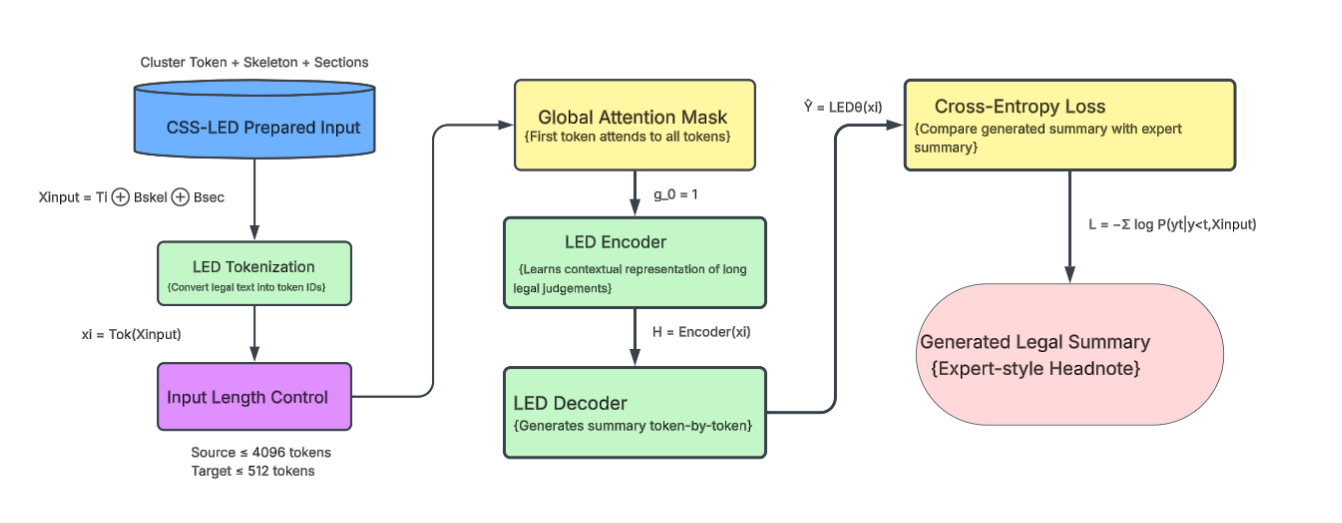
\includegraphics[width=0.9\textwidth]{Led.png}
\caption{\textbf{LED-based abstractive summarization architecture for generating legal judgment summaries from structured long-document input.}}
\label{fig:led_architecture}
\vspace{-2mm}
\end{figure}

The diagram above shows how the encoded data is decoded by LED encoder.

In the proposed system, the pretrained model used is: \texttt{allenai/led-base-16384} ~\cite{b21}

The maximum source length is fixed as:

\begin{equation}
L_{\text{src}} = 4096
\end{equation}

and the maximum target summary length is fixed as:

\begin{equation}
L_{\text{tgt}} = 512
\end{equation}

In the case that input sequence is longer than max source length, first keep cluster token and salient skeleton since they carry very useful instruction information. The rest of document block will be trimmed

\begin{equation}
X_i^{\text{input}} =
T_{\text{cluster}} \oplus B_{\text{skel}} \oplus \operatorname{Truncate}(B_{\text{doc}})
\end{equation}

During generation, global attention is applied to the first token so that the model can use it as a global information point:

\begin{equation}
g_j =
\begin{cases}
1, & j = 0, \\
0, & \text{otherwise}.
\end{cases}
\end{equation}

where \(g_j\) denotes the global attention mask for the \(j^{th}\) token.

The model generates the summary token by token in an autoregressive manner:

\begin{equation}
\hat{Y}_i =
\{\hat{y}_1, \hat{y}_2, \ldots, \hat{y}_T\}
\end{equation}

where each generated token depends on the input sequence and the previously generated tokens:

\begin{equation}
\hat{y}_t =
\arg\max_{y_t} P\left(y_t \mid y_{<t}, X_i^{\text{input}}\right)
\end{equation}

In conclusion, LED creates an abstractive summary in short text using combined structure judgment, sentence salience skeleton and semantic case signal to handle long legal document and reserve necessary legal information for generation.

\subsection{Training and Evaluation}
Once the final input format is ready the data is written into JSONL files for training, validation and testing. The format of each JSONL record will consist of the case id, final input text and target gold summary. The training file is utilized for the purpose of fine-tuning the LED model, the validation file is utilized to keep track of the model performance during the training phase and the test file is used for the final assessment.

Let the final training, validation, and test sets be represented as:

\begin{equation}
\mathcal{D}_{\text{train}} =
\left\{ \left(X_i^{\text{input}}, Y_i\right) \right\}_{i=1}^{N_{\text{train}}}
\end{equation}

\begin{equation}
\mathcal{D}_{\text{val}} =
\left\{ \left(X_i^{\text{input}}, Y_i\right) \right\}_{i=1}^{N_{\text{val}}}
\end{equation}

\begin{equation}
\mathcal{D}_{\text{test}} =
\left\{ \left(X_i^{\text{input}}, Y_i\right) \right\}_{i=1}^{N_{\text{test}}}
\end{equation}

where \(X_i^{\text{input}}\) denotes the final model input, and \(Y_i\) denotes the expert-written reference summary.

Prior to training the source and target summaries are tokenised with the LED tokenizer. We constrain source input to 4096 and target summary to 512.

\begin{equation}
\operatorname{Tok}\left(X_i^{\text{input}}\right) \leq 4096
\end{equation}

\begin{equation}
\operatorname{Tok}(Y_i) \leq 512
\end{equation}

The LED model is fine-tuned using the standard sequence-to-sequence training objective commonly used in neural abstractive summarization ~\cite{b7,b8,b9,b10}. Let \(y_t\) be the target token at decoding step \(t\), and let \(p_{\theta}(y_t \mid y_{<t}, X_i^{\text{input}})\) be the probability predicted by the model. The training loss is computed as:

\begin{equation}
\mathcal{L}
=
-\sum_{t=1}^{L_{\text{tgt}}}
\mathbb{I}(y_t \neq -100)
\log p_{\theta}\left(y_t \mid y_{<t}, X_i^{\text{input}}\right)
\end{equation}

where \(\mathbb{I}(\cdot)\) is an indicator function, and \(-100\) is used to ignore padding tokens during loss calculation.

During summary generation, global attention is applied to the first token of the input sequence:

\begin{equation}
g_j =
\begin{cases}
1, & j = 0, \\
0, & \text{otherwise}.
\end{cases}
\end{equation}

where \(g_j\) is the global attention mask for the \(j^{th}\) token. This helps the model use the first token as a global reference point while processing the long input sequence.

The final summary is generated using beam search decoding:

\begin{equation}
\hat{Y}_i =
\arg\max_{Y}
P_{\theta}\left(Y \mid X_i^{\text{input}}\right)
\end{equation}

where \(\hat{Y}_i\) is the generated summary. Beam search keeps multiple possible output sequences during decoding and selects the most likely summary.

The summaries produced by the model are evaluated against the human-written reference summaries using ROUGE-1, ROUGE-2 and ROUGE-L measures ~\cite{b43}. ROUGE-1 calculates unigram overlap, ROUGE-2 calculates bigram overlap and ROUGE-L measures longest common subsequence similarity.

For ROUGE-N, the score is computed using n-gram overlap between the generated summary \(\hat{Y}_i\) and the reference summary \(Y_i\):

\begin{equation}
\mathrm{ROUGE}\text{-}N =
\frac{
\sum_{\mathrm{gram}_n \in Y_i} \operatorname{Count}_{\text{match}}(\mathrm{gram}_n)
}{
\sum_{\mathrm{gram}_n \in Y_i} \operatorname{Count}(\mathrm{gram}_n)
}
\end{equation}

where \(\operatorname{Count}_{\text{match}}(\mathrm{gram}_n)\) is the number of matched n-grams between the generated and reference summaries.

For ROUGE-L, the longest common subsequence is used:

\begin{equation}
\mathrm{ROUGE}\text{-}L =
\frac{
\operatorname{LCS}(Y_i,\hat{Y}_i)
}{
|Y_i|
}
\end{equation}

where \(\operatorname{LCS}(Y_i,\hat{Y}_i)\) denotes the longest common subsequence between the reference summary and the generated summary.

In the experimental part, the newly-put-forward CSS-LED model is contrasted with several baseline models based on the above evaluation measures to quantify whether structure-aware representation and salience skeleton guidance benefit summarization quality better than previous summarization methods.

\section{Experimental Setup}

\subsection{Dataset Description}
The experiments are performed on the IN-ABS dataset of Indian legal judgments and gold-standard, human-written headnotes ~\cite{b1}. Each data sample in the dataset consists of a source document (judgment) and a corresponding gold summary (headnote). In this work, the source legal judgment is denoted by $X_i$ and the expert-written headnote is denoted by $Y_i$. Accordingly, the task is formulated as an abstractive legal judgment summarization problem, where the objective is to train a model that generates a concise legal summary $\hat{Y}_i$ given the source legal judgment document $X_i$.

For the experiments, the training cases are limited to a capped portion of 6000 cases which can maintain data coverage and reasonable computation amount. Out of the 6000 cases, we held out 10\% for validation and used the rest for fine-tuning the model. Hence, we have now 5400 cases for training and 600 cases for validation. We did not change the standard IN-ABS split and it was only used for testing. The dataset split for the experiments can be seen in Table~\ref{tab:dataset_split}.

\begin{table}[H]
\centering
\caption{Dataset split used in the experimental setup.}
\begin{tabular}{lcl}
\hline
Split & Number of Samples & Purpose \\
\hline
Training & 5400 & Model fine-tuning \\
Validation & 600 & Hyperparameter monitoring \\
Test & Standard IN-ABS test split & Final evaluation \\
\hline
\end{tabular}
\label{tab:dataset_split}
\end{table}

\subsection{Experimental Environment}
All the experiments were developed in Python, using PyTorch along with the Hugging Face Transformers library. The data preparation, preprocessing, input building, tokenization, model fine-tuning, evaluation scripts were all run in a Kaggle GPU environment. The experiments were run with NVIDIA P100 GPU runtime when training the long-document summarization model based on LED ~\cite{b21}.

Since legal judgments are extremely long, memory optimization was required when training the LED-based long-document summarization model ~\cite{b21}. Therefore memory optimization has been applied during the training. The maximum source length is 4096 tokens, and the target summary length is 512 tokens. Mixed-precision training has been turned on so as to limit GPU memory usage. Gradient check pointing has been turned on to make the intermediate activations can be recomputed during the back propagation instead of being fully stored into the memory. The gradients were accumulated by using small per-device batch size to gain stable effective batch size that do not break GPU memory limitations.

The present experimental configuration enabled processing long legal judgment inputs with the LED-based summarization model under computational limitations of a single-GPU notebook environment.

\subsection{Data Preparation Protocol}

IN-ABS was first processed to get matched judgment-summary pair of cases. The source judgment file was matched with its summary from expert, the headnote file with the help of the case identifier. Cases both for which the source judgment and summary are available were selected and the remaining cases were discarded to ensure that each case has the complete source-target pair for abstractive summarization task.

Following the pairing stage, each of the raw judgments was passed through a domain-specific pipeline of cleaning steps to eliminate repeated court metadata, page numbers, headers, footers, incomplete line breaks, irregular punctuation and boilerplate legal text, etc., and to make them more standardized, to prevent non-substantive formatting noise from taking space in the model input space.

Then the normalized judgment was divided into the five standard legal categories; facts, issue, arguments, reasoning and judgment/order. The section mappings were extracted by means of legal heading patterns whenever possible. If there are no obvious headings, the positional Fallback Strategy were used to keep the original order of the whole judgment, which results in a document structure where sections are explicitly demarcated.

In following section structuring and semantic case conditioning was carried out. An extract from each of the judgment texts were represented with the MiniLM sentence embedding model ~\cite{b41}. Dense embeddings generated from this model were clustered with K-Means, and an semantic cluster ID assigned to each case. This case specific cluster label was then turned into a cluster token and concatenated onto the model input.

Last, gold-summary-guided salient skeleton was extracted with the salience value calculation based on TF-IDF cosine similarity. The source judge sentences and gold summary sentences were translated into TF-IDF vectors, and the sentences which had the highest TF-IDF similarity with gold summary sentences were chosen as salient sentences. The extracted salient sentences were reordered into the order in source document to reserve legal flows. The finally generated LED input included the cluster token, the salient skeleton block and the structured document block.

\begin{table}[H]
\centering
\caption{Data preparation stages used before LED fine-tuning.}
\begin{tabular}{ll}
\hline
Stage & Description \\
\hline
Pair creation & Match each judgment with its gold summary \\
Text cleaning & Remove formatting noise, metadata, and boilerplate text \\
Section segmentation & Map judgment into facts, issues, arguments, reasoning, and final order \\
Semantic clustering & Assign a cluster token using MiniLM and K-Means \\
Skeleton extraction & Select salient source sentences using TF-IDF similarity \\
Input construction & Combine cluster token, skeleton block, and structured document \\
\hline
\end{tabular}
\label{tab:data_preparation}
\end{table}

\subsection{Model Configuration}
The CSS-LED framework was put in place on top of a long document encoder-decoder architecture that provided the abstractive summarization backbone. LED encoder decoder model was chosen because of its support for longer sequences that the classical transformer encoder decoder has. MiniLM embedding was implemented as case semantic representation while using K-Means clustering to allocate a case to a certain semantic cluster label.

For the salience guidance, the skeleton extraction module selected source sentences by TF-IDF cosine similarity between the judgment sentence and the gold summary sentence. The selected skeleton sentences were then concatenated with the semantic cluster token and the document block structure and then fed into the LED model.The major hyperparameter settings are displayed in Table~\ref{tab:hyperparameter_setting}.

\begin{table}[H]
\centering
\caption{Hyperparameter settings used for CSS-LED experiments.}
\begin{tabular}{ll}
\hline
Parameter & Value \\
\hline
Backbone model & allenai/led-base-16384 \\
Embedding model & all-MiniLM-L6-v2 \\
Clustering method & K-Means \\
Number of clusters & 6 \\
Maximum source length & 4096 tokens \\
Maximum target length & 512 tokens \\
Skeleton sentence limit & 60 sentences \\
Top-K source sentences per summary sentence & 3 \\
Similarity threshold & 0.10 \\
Learning rate & $2 \times 10^{-5}$ \\
Weight decay & 0.01 \\
Epochs & 2 \\
Per-device batch size & 1 \\
Gradient accumulation steps & 4 \\
Effective batch size & 4 \\
Loss function & Masked cross-entropy \\
\hline
\end{tabular}
\label{tab:hyperparameter_setting}
\end{table}

\subsection{Baseline Models} 
The performance impact of our structure-aware and salience-guided input formulation is assessed by using the CSS-LED model against two extractive and abstractive baseline models. We introduce the two extractive baselines for exploring if sentence extraction is effective enough for the generation of compressed legal headnotes. These techniques largely choose some high-salience sentences from the source judgement instead of fully abstractive generation.

We also introduce a plain LED baseline to investigate the capability of the long-context modeling for summarization in legal domain whether is sufficient or not, which simply employs the LED backbone without the proposed section-aware format, semantic cluster token, and salience skeleton guidance, making it possible to differentiate the effect of the proposed components.

\begin{table}[H] \centering \caption{Baseline models considered for experimental comparison.} \begin{tabular}{lll} \hline Model & Type & Purpose \\ \hline TextRank ~\cite{b11} & Extractive & Graph-based sentence ranking baseline \\ SBERT + K-Means & Extractive & Semantic clustering-based sentence selection \\ SBERT + TF-IDF + K-Means & Extractive & Lexical-semantic hybrid baseline \\ SBERT Centroid & Extractive & Centroid-based sentence selection \\ Plain LED ~\cite{b21} & Abstractive & Long-document baseline without structure/skeleton \\ CSS-LED & Abstractive & Proposed full framework \\ \hline \end{tabular} \label{tab:baseline_models} \end{table} 

Also, In terms of the effectiveness, we analyze how much benefit is contributed by the structure-aware and salience-guided input formulation by comparing CSS-LED with common extractive and abstractive baseline models used in legal and generic summarization contexts ~\cite{b1, b2, b11, b18, b21}.

\subsection{Evaluation Metrics}

The produced summarization of the legal documents were tested by applying ROUGE metric suite ~\cite{b43}. ROUGE tests the created summary with that of expert made in headnote in terms of the degree of common word as well as structural elements. Here, ROUGE-1, ROUGE-2 and ROUGE-L were mainly chosen.

ROUGE-1 computes the unigram overlap between the generated and reference summaries and focuses primarily on what proportion of the content of the expert-written headnote is captured by the model generated output. ROUGE-2 calculates bigram overlaps to provide some measure of local coherence at the phrase level. ROUGE-L looks at the length of the longest common subsequence of the generated and reference summary which measures sequentiality and structure.

The F1-score of the Rouge, recall of the Rouge, and the Rouge precision score have been provided for every Rouges Metric. Precision computes the percentage of the content that exists in the generated summary out of the total content in the reference summary and, in the same way, the recall represents the percentage of the total reference content that is covered by the generated summary output. The metrics to be considered during the Experiments are present in the Table~\ref{tab:evaluation_metrics} below.

\begin{table}[H]
\centering
\caption{Evaluation metrics used for summary assessment.}
\begin{tabular}{ll}
\hline
Metric & Purpose \\
\hline
ROUGE-1 & Measures unigram overlap and content coverage \\
ROUGE-2 & Measures bigram overlap and local coherence \\
ROUGE-L & Measures longest common subsequence and structural similarity \\
Precision & Measures relevance of generated summary content \\
Recall & Measures coverage of reference summary content \\
F1-score & Balances precision and recall \\
\hline
\end{tabular}
\label{tab:evaluation_metrics}
\end{table}

\section{Results}
\subsection{Performance of the Proposed CSS-LED Model}

Firstly, the performance of the designed CSS-LED model is compared on the IN-ABS test set in terms of ROUGE precision, recall and F1-score. Table~\ref{tab:css_led_performance} shows the reported results.

\begin{table}[H]
\centering
\caption{Performance of the proposed CSS-LED model on the IN-ABS test set.}
\begin{tabular}{lccc}
\hline
Metric & Precision & Recall & F1-score \\
\hline
ROUGE-1 & 72.40 & 39.95 & 50.63 \\
ROUGE-2 & 40.45 & 22.34 & 28.48 \\
ROUGE-L & 43.04 & 23.64 & 30.12 \\
\hline
\end{tabular}
\label{tab:css_led_performance}
\end{table}

The CSS-LED model performance on IN-ABS test set can be seen from table~\ref{tab:css_led_performance}. The F1-score of 50.63 for ROUGE-1 indicates the generated summary retains a substantial amount of important content at the unigram level of the ground-truth headnotes. The ROUGE-2 F1-score of 28.48 indicates that the model also retains good amount of shared phrasal content, but naturally it’s harder since the model can rephrase legal statements. Finally, the ROUGE-L F1-score of 30.12 indicates that the produced summary sequence exhibits a reasonable amount of similarity with the ground-truth summary sequence.

Across all three ROUGE metrics, precision scores are consistently greater than the recall scores, indicating that our generated summaries are relatively concise and consist of numerous terms of the reference summary, but possibly missing some facts in the references. All in all, the experimental results show that CSS-LED model can produce concise legal summary based on lengthy judicial opinions, and retain the key legal facts in the generated summaries.

\subsection{Comparison with Implemented Baselines}

In Table~\ref{tab:implemented_baseline_comparison}, we show the results obtained by the CSS-LED model along with a few other existing implementations, in order to study the impact of structure-aware representation and salience-guided input construction. The other implementations consist of extractive models like SBERT, TF-IDF, K-Means clustering, centroid selection, and TextRank, in addition to a Plain LED model that only incorporates the standard input without our proposed salience and structure-awareness.

\begin{table}[H]
\centering
\caption{Comparison of CSS-LED with implemented baseline models on the IN-ABS dataset.}
\resizebox{\textwidth}{!}{
\begin{tabular}{lccccccccc}
\hline
\multirow{2}{*}{Model} & \multicolumn{3}{c}{ROUGE-1} & \multicolumn{3}{c}{ROUGE-2} & \multicolumn{3}{c}{ROUGE-L} \\
\cline{2-10}
& Prec & Recall & F1 & Prec & Recall & F1 & Prec & Recall & F1 \\
\hline
SBERT + TF-IDF + K-Means & 15.18 & 38.98 & 19.57 & 15.04 & 14.95 & 15.94 & 7.91 & 13.48 & 20.24\\
SBERT + K-Means & 14.18 & 38.48 & 17.57 & 5.04 & 14.65 & 5.94 & 7.71 & 19.48 & 10.24 \\
SBERT Centroid & 13.72 & 8.44 & 16.73 & 14.50 & 8.33 & 5.90 & 8.01 & 8.44 & 10.12 \\
TextRank ~\cite{b11} & 14.07 & 40.48 & 17.37 & 6.07 & 16.39 & 6.74 & 8.31 & 19.48 & 10.7 \\
Plain LED ~\cite{b21} & 16.79	& 38.99	 & 18.58 & 4.61	& 8.82 & 4.60 & 9.87 & 22.39 & 11.51 \\
\hline
\textbf{CSS-LED} & \textbf{72.40} & \textbf{42.95} & \textbf{50.63} & \textbf{40.45} & \textbf{22.34} & \textbf{28.48} & \textbf{43.04} & \textbf{23.64} & \textbf{30.12} \\
\hline
\end{tabular}}
\label{tab:implemented_baseline_comparison}
\end{table}

The CSS-LED model outperforms all of the implemented baseline methods across all three ROUGE variants in terms of the F1-score as presented in Table~\ref{tab:implemented_baseline_comparison}. The results of extractive baselines, TextRank and SBERT based clustering methods are of very high precision and low recall because they only cover a very few overlapping text spans and cannot capture the reference well. SBERT Centroid can cover slightly better than other extractive baselines with respect to recall, but the overall F1 score still lags far behind our method.

Poor Performance of the Plain LED baseline even. Long context generation is not alone capable of summary for judgment. The LED could accept more input, yet stronger guides were still needed to detect which text span within the longer judgment had legal significance. Our CSS-LED increased both the recall and F1-score, since the model was aware of the structure (salience skeleton) and the content-awareness information (section representation of the judgment). Hence, the model was guided to attend to important facts, reasoning, and the judgment decision rather than processing the judgment as a sequence of texts.

\begin{figure*}[!t]
\centering

\begin{subfigure}{0.32\textwidth}
    \centering
    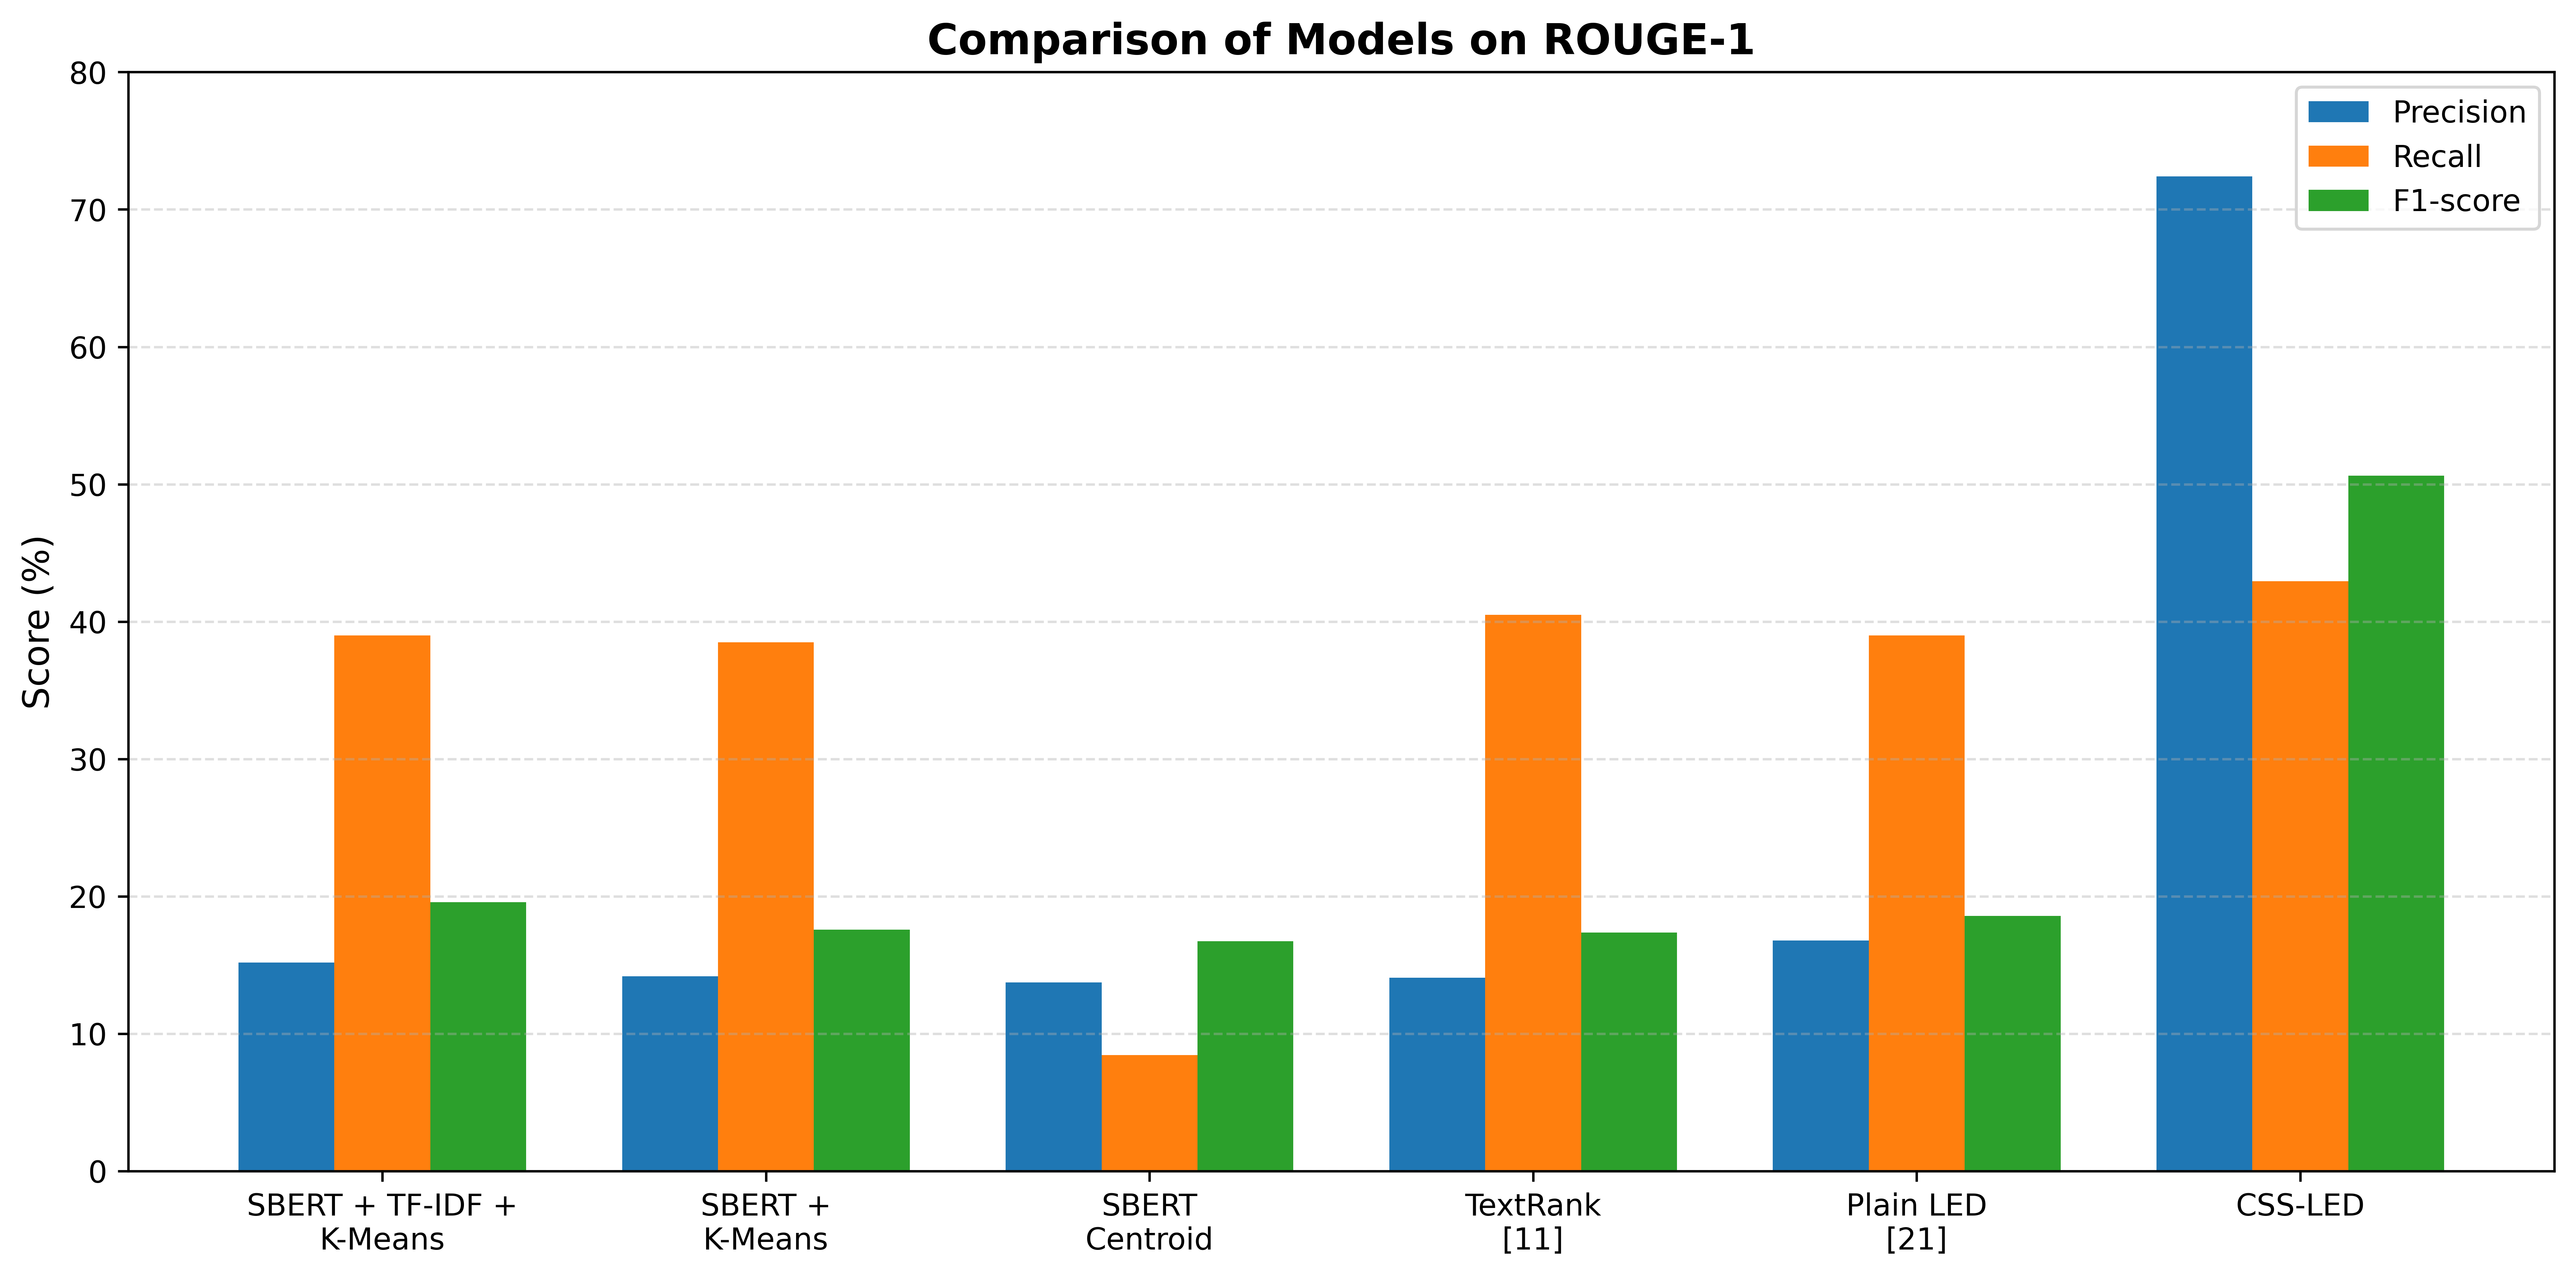
\includegraphics[width=\linewidth]{rouge1_comparison.png}
    \caption{ROUGE-1}
\end{subfigure}
\hfill
\begin{subfigure}{0.32\textwidth}
    \centering
    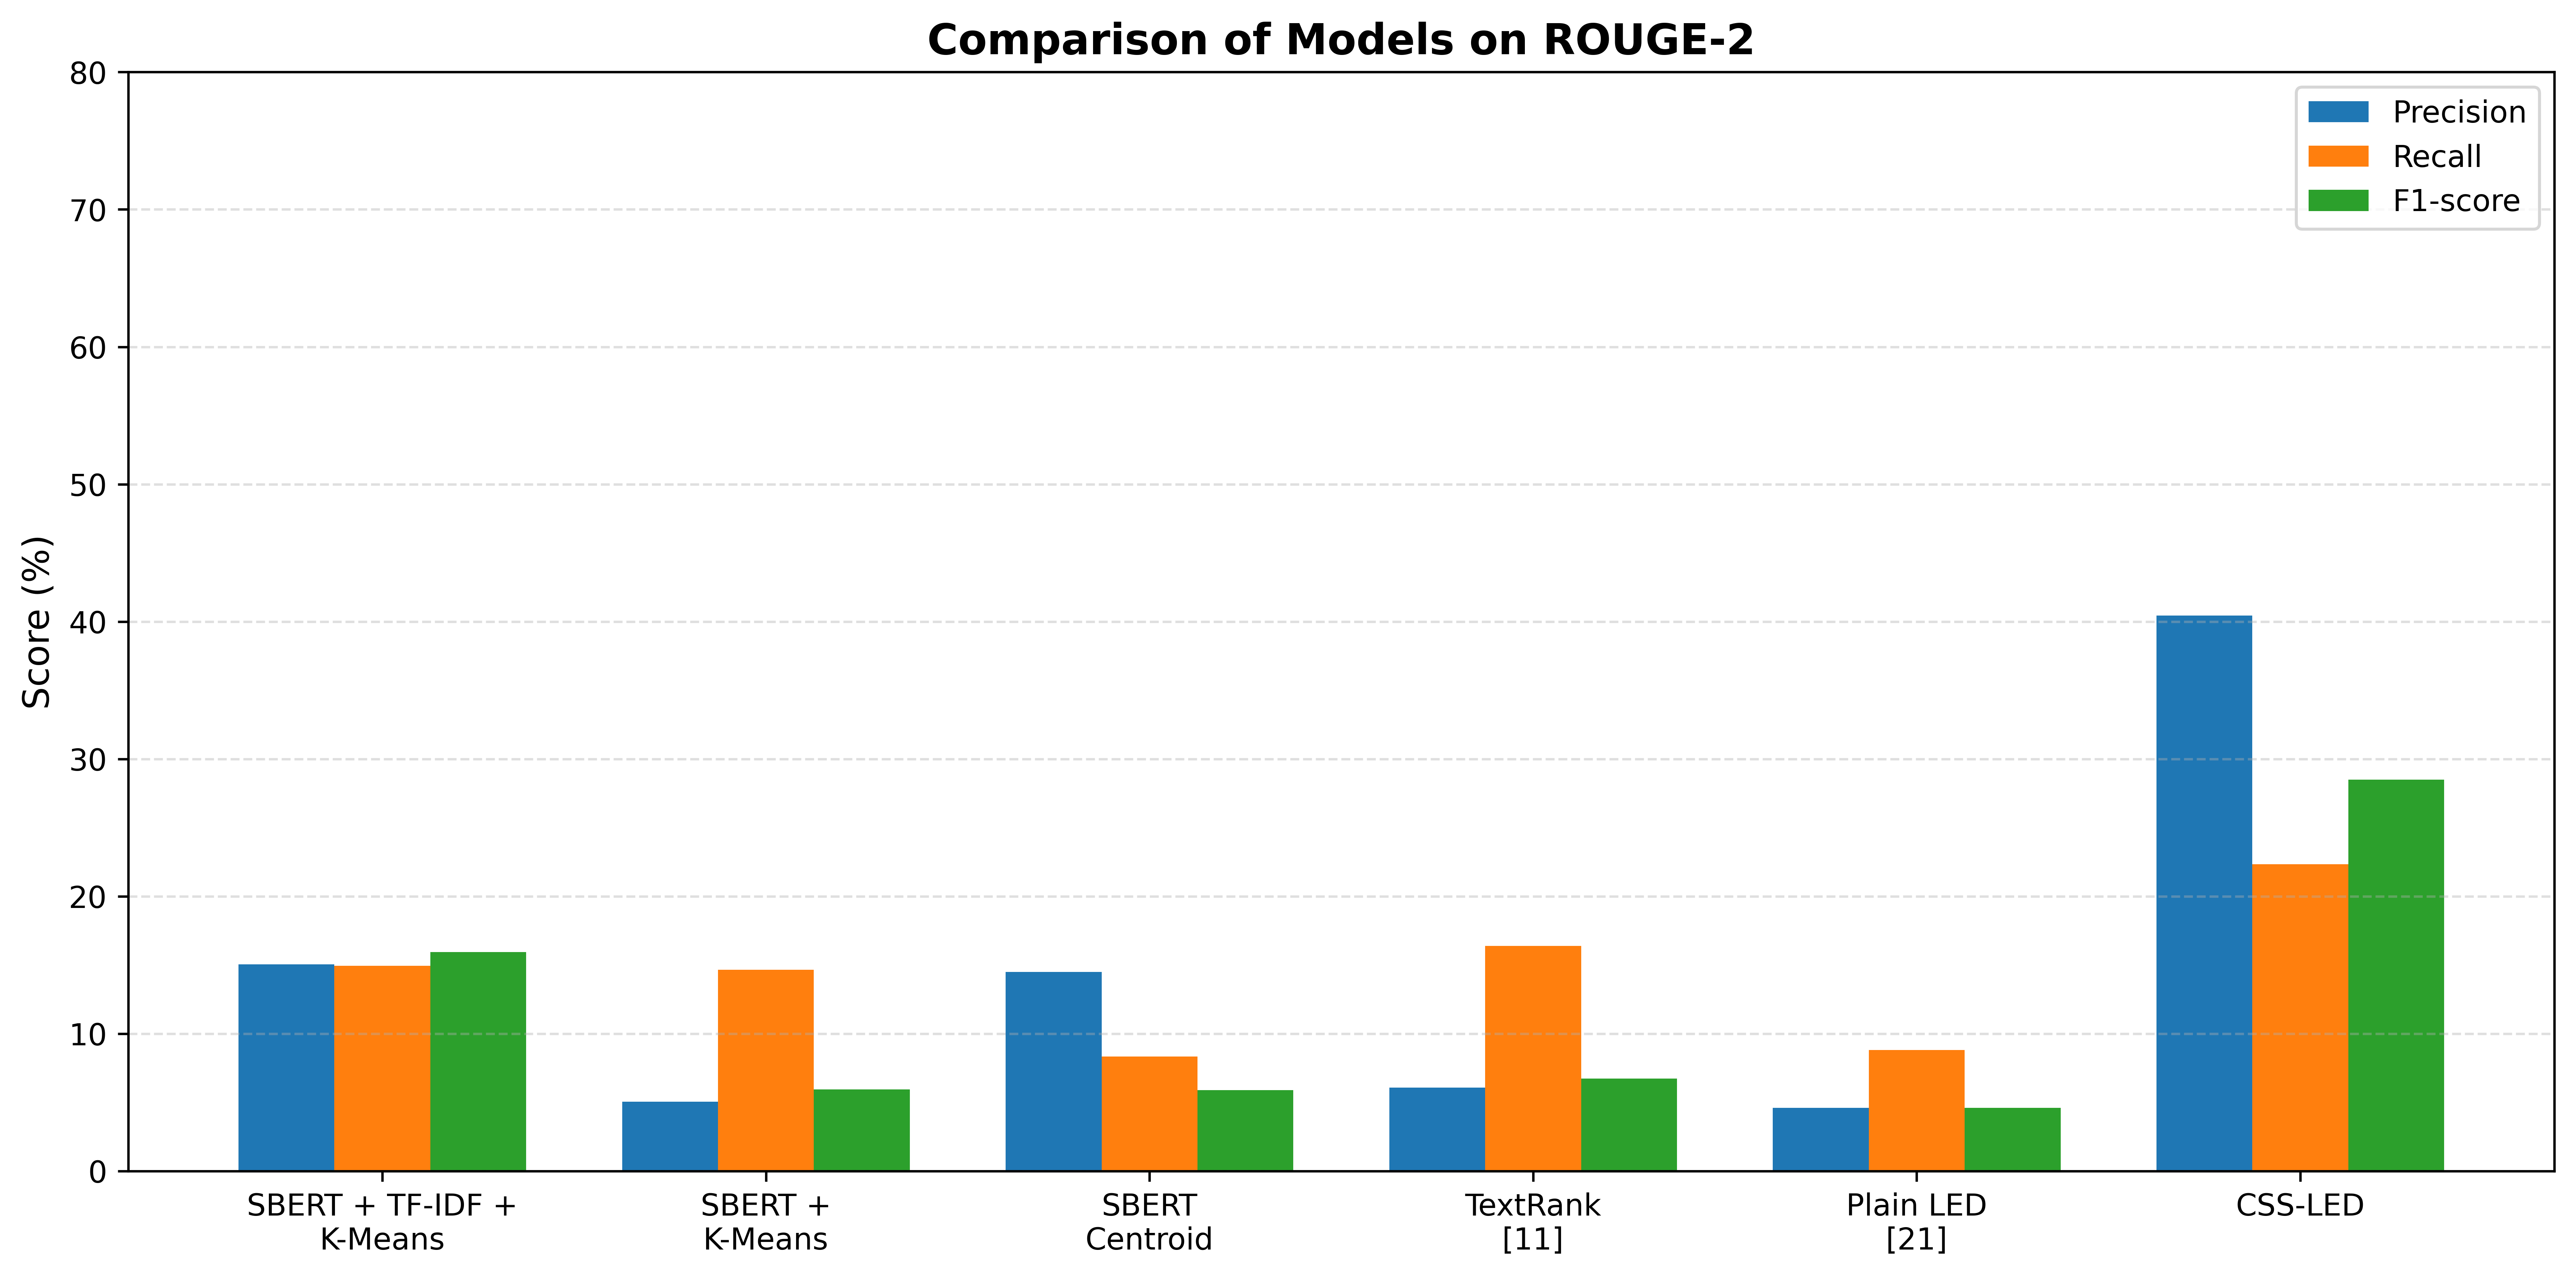
\includegraphics[width=\linewidth]{rouge2_comparison.png}
    \caption{ROUGE-2}
\end{subfigure}
\hfill
\begin{subfigure}{0.32\textwidth}
    \centering
    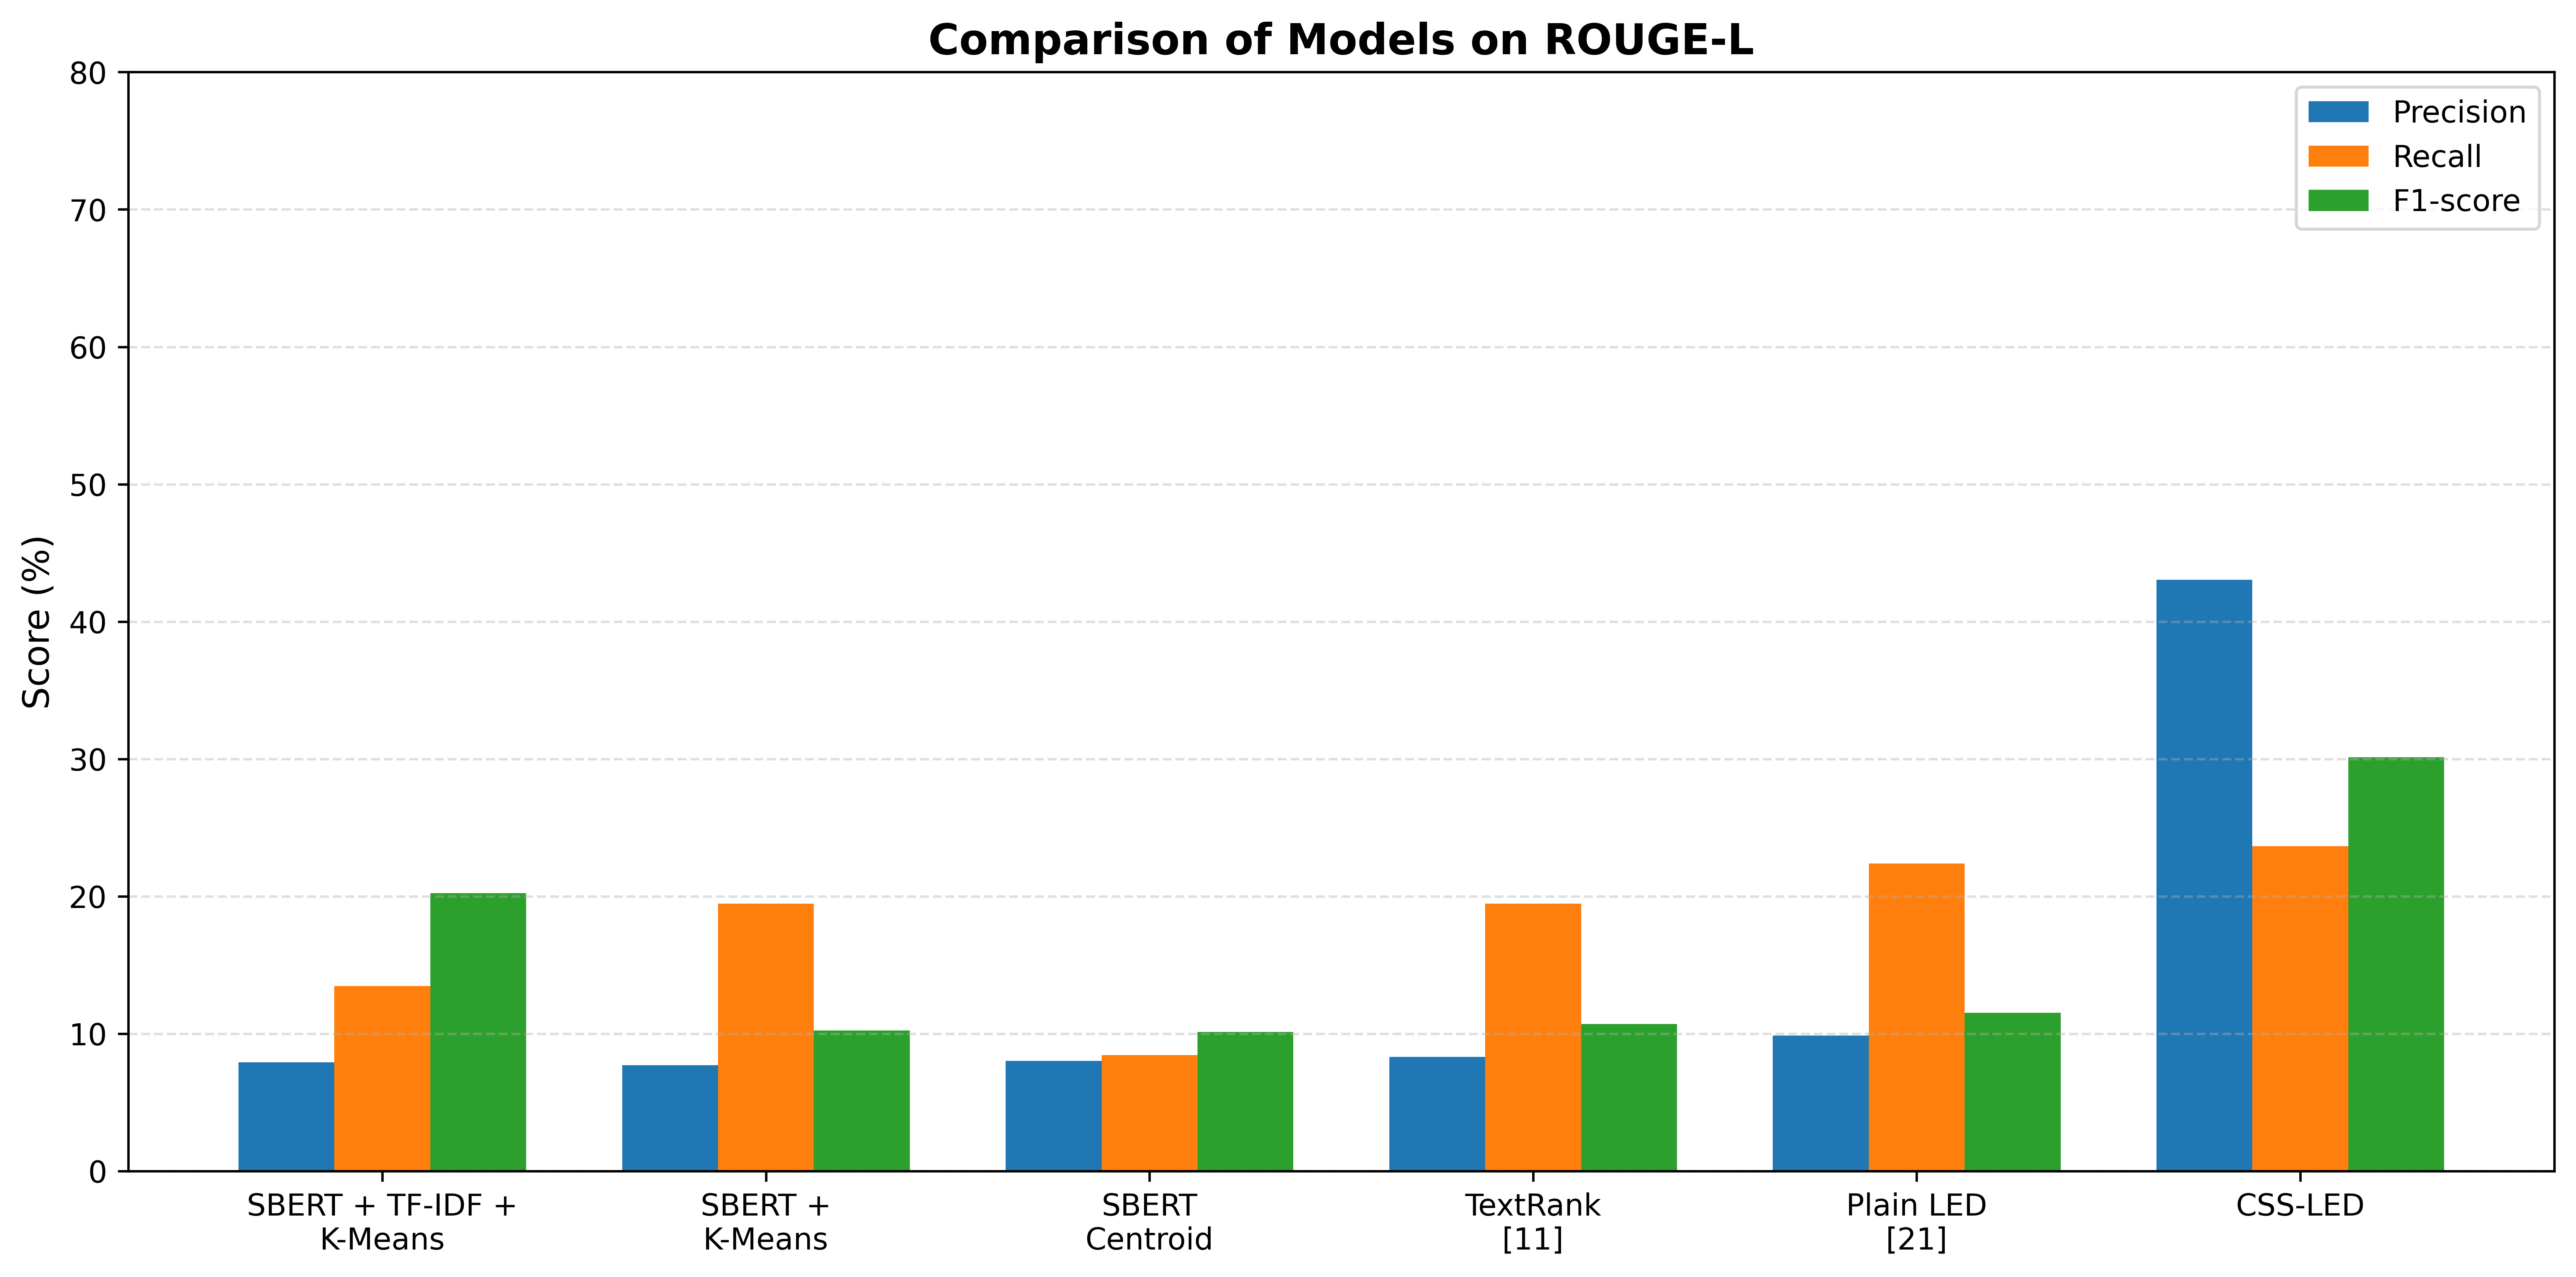
\includegraphics[width=\linewidth]{rougel_comparison.png}
    \caption{ROUGE-L}
\end{subfigure}

\caption{Performance comparison of CSS-LED with implemented baseline models on the IN-ABS dataset.}
\label{fig:implemented_baseline_comparison}
\end{figure*}

Figure~\ref{fig:implemented_baseline_comparison} visualizes the comparison with implemented baselines across ROUGE-1, ROUGE-2, and ROUGE-L using precision, recall, and F1-score.

\subsection{Comparison with Existing Work}
We also show how the CSS-LED model compares to several other well-cited extractive and abstractive models for legal judgment summarization on the IN-ABS dataset. The experimental results are listed in Table~\ref{tab:prior_work_full}.

\begin{table}[H]
\centering
\caption{Comparison with Prior Work on IN-ABS (ROUGE Precision, Recall, and F1)}
\label{tab:prior_work_full}
% \resizebox{\textwidth}{!} ensures the 11 columns do not spill over the page margins
\resizebox{\textwidth}{!}{
\begin{tabular}{ll ccc ccc ccc}
\toprule
\multirow{2}{*}{\textbf{Model}} & \multirow{2}{*}{\textbf{Type}} & \multicolumn{3}{c}{\textbf{ROUGE-1}} & \multicolumn{3}{c}{\textbf{ROUGE-2}} & \multicolumn{3}{c}{\textbf{ROUGE-L}} \\
\cmidrule(lr){3-5} \cmidrule(lr){6-8} \cmidrule(lr){9-11}
& & \textbf{Prec} & \textbf{Recall} & \textbf{F1} & \textbf{Prec} & \textbf{Recall} & \textbf{F1} & \textbf{Prec} & \textbf{Recall} & \textbf{F1} \\
\midrule

Case Summarizer \cite{b2} & Extractive (U)    & 52.69 & 36.11 & 40.74 & 20.82 & 14.51 & 16.30 & 26.97 & 18.36 & 20.72 \\
SummaRunner \cite{b36}      & Extractive (S)    & 55.47 & 39.20 & 48.41 & 22.25 & 18.29 & 19.24 & 25.45 & 21.25 & 22.20 \\
Legal-Pegasus \cite{b10, b11}   & Abstractive (Pre) & 69.52 & 21.41 & 32.1 & 27.81 & 8.35 & 12.58 & 37.73 &	11.45 & 17.21 \\
BART\_MCS \cite{b8, b11}        & Abstractive (FT)  & 69.60 & 8.55 & 14.99 & 30.18 & 3.35 & 5.92 & 42.10 & 5.5 & 9.69 \\
Legal-LED (FT) \cite{b21, b11}  & Abstractive (FT)  & 61.61 & 22.17 & 31.88 & 21.37 & 7.41 & 10.76 & 33.52 & 11.87 & 17.13 \\

\midrule
\textbf{CSS-LED (Ours)} & Abstractive (FT) & \textbf{72.40} & \textbf{39.95} & \textbf{50.63} & \textbf{40.45} & \textbf{22.34} & \textbf{28.48} & \textbf{43.04} & \textbf{23.64} & \textbf{30.12} \\

\bottomrule
\end{tabular}
}
\end{table}

For comparison with prior work, we include representative extractive and abstractive legal summarization models reported in earlier legal judgment summarization studies, including CaseSummarizer, SummaRunner, Legal-Pegasus, BART-based models, and Legal-LED ~\cite{b1, b2, b4, b8, b10, b21, b36}.


Table~\ref{tab:prior_work_full} summarizes the performance of CSS-LED compared with the current extract and abstractive methods on the IN-ABS dataset. CSS-LED achieves top performances on ROUGE-1, ROUGE-2, and ROUGE-L. In particular, it produces a slight increase in ROUGE-1 F1 when comparing with SummaRunner but a more substantial increase in ROUGE-2 and ROUGE-L F1's. This shows that the proposed method is capable of capturing important information and also improving phrase level correspondence and sequential correlation between candidate summaries and the reference summaries.

This comparison further indicates that CSS-LED provides gains over abstractive baselines including Legal-Pegasus, BART MCS, and Legal-LED. This is largely attributable to the proposed approach that does not rely solely on the backbone model generation capability but enriches with the guidance signals from legal section tags, case semantic condition and summary-aligned salient sentences that help focus the generation on legally-relevant fact, argument, reasoning and conclusion.

\begin{figure}[H]
\centering
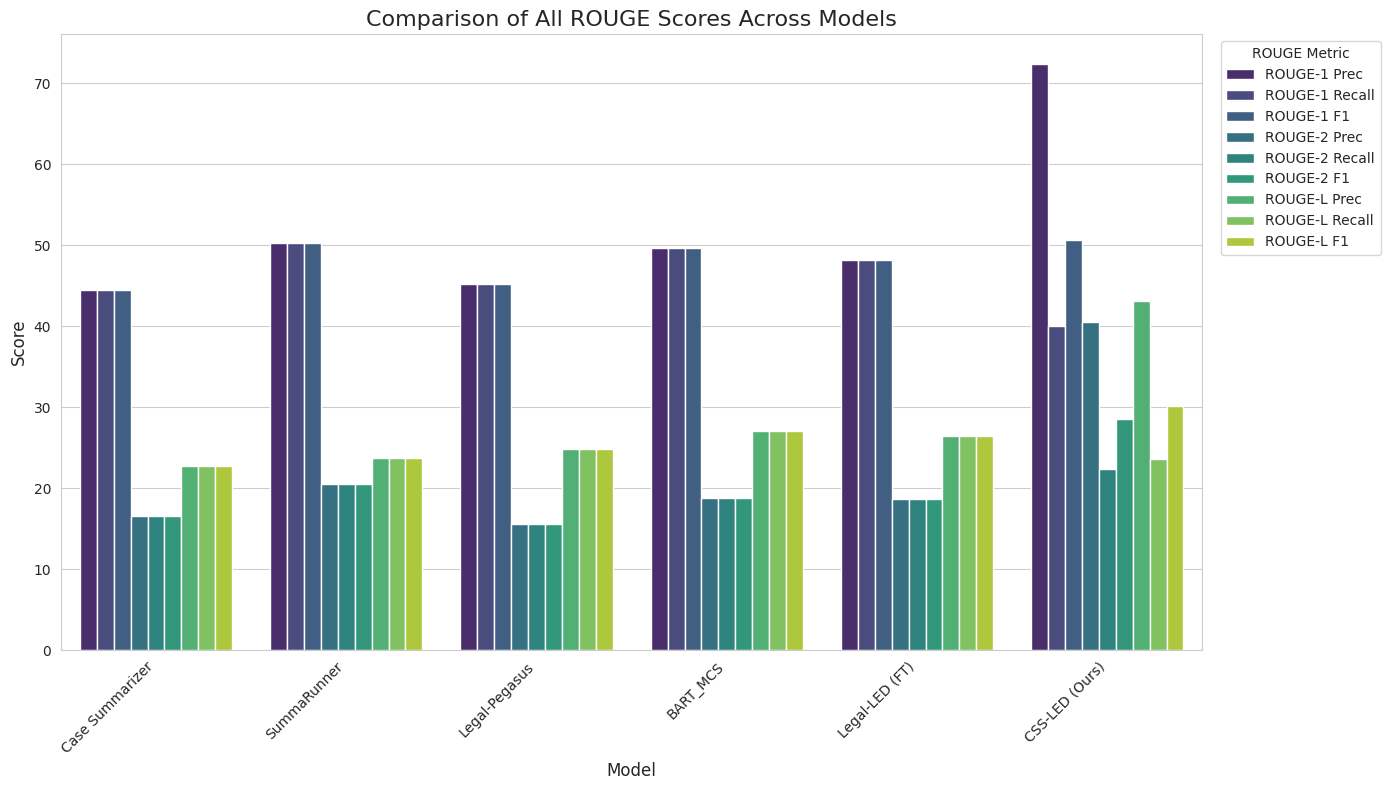
\includegraphics[width=0.90\textwidth]{MCOMP.png}
\caption{Comparison of CSS-LED with existing methods on the IN-ABS dataset.}
\label{fig:prior_work_comparison}
\end{figure}

\subsection{Sensitivity Analysis}
We will summarize the sensitivity of our CSS-LED model with different source-token limit. As legal decisions tend to be long, the token limit impacts what kind of information about factual background, reasoning, argumentation and final ruling are provided to the model. Thus we explore the efficacy of the suggested formulation as the budget gets squeezed.

\begin{table}[H]
\centering
\caption{Sensitivity analysis of CSS-LED under different source-token limits.}
\begin{tabular}{lcccc}
\hline
Source Token Limit & ROUGE-1 & ROUGE-2 & ROUGE-L & ROUGE-Lsum \\
\hline
512 & 49.37 & 27.00 & 28.64 & 45.60 \\
1024 & 48.48 & 26.94 & 28.56 & 44.71 \\
2048 & 49.66 & 27.45 & 29.04 & 45.87 \\
4096 & 49.72 & 27.67 & 29.29 & 46.11 \\
8192 & 50.39 & 27.72 & 29.51 & 46.62 \\
16000 & 50.39 & 27.72 & 29.51 & 46.62 \\
\hline
\end{tabular}
\label{tab:token_sensitivity}
\end{table}

Table~\ref{tab:token_sensitivity} summarizes the results when varying the number of source tokens, we used, in which case CSS-LED still shows promising scores for input sequences as short as 512 and 1024 tokens. This supports that placing the salience skeleton close to the beginning of the input saves the key information relevant for the task both in terms of facts and law.

The performance gets higher step by step as token limit changes from 2048 to 8192. It reaches to the best when token limit is 8192 tokens. Scores are 50.39 ROUGE-1, 27.72 ROUGE-2, 29.51 ROUGE-L, 46.62 ROUGE-Lsum. After that, the scores at 16000 tokens are the same as that of 8192 tokens, which means input-ordering doesn’t contribute any further when the limit is larger than 8192. On the whole, this sensitivity analysis demonstrates that the input-ordering proposed can provide additional benefits when the input token is restricted within limits for long document summarization on the legal judgment dataset.

\subsection{Qualitative Case Study}
Besides the ROUGE-based evaluation, a tiny qualitative case study is presented to inspect how the proposed CSS-LED model summarises the cases. Five case studies from the IN-ABS test set are randomly chosen. Both gold and generated summaries are compared in Table~\ref{tab:qualitative_study}.

\begin{longtable}{c c p{10.5cm}}
\caption{Representative Qualitative Comparison of Gold and Generated Summaries on the IN-ABS Test Set}
\label{tab:qualitative_study} \\

\toprule
\textbf{Case No.} & \textbf{Type} & \textbf{Summary} \\
\midrule
\endfirsthead

\multicolumn{3}{c}%
{{\bfseries \tablename\ \thetable{} -- continued from previous page}} \\
\toprule
\textbf{Case No.} & \textbf{Type} & \textbf{Summary} \\
\midrule
\endhead

\midrule \multicolumn{3}{r}{{Continued on next page}} \\
\endfoot

\bottomrule
\endlastfoot

\multirow{2}{*}{2440} & Gold Summary &
Industrial dispute on fixation of wages and bonus for 1962–64. 
Tribunal examined regional wage structures and comparable industries. 
Minimum wage revision in respondent mills was considered justified. 
Price index was relevant in wage determination. 
Tribunal avoided automatic linking of wages to price fluctuations. 
Workers could seek revision later if needed. 
Dispute centered on fairness of wage fixation. \\
\cmidrule{2-3}
 & Generated Summary &
Tribunal compared wages with similar regional industries. 
Minimum wage principle was applied in wage fixation. 
Multiple industrial disputes were reviewed. 
Wages were not directly tied to price index changes. 
Clerical staff dearness allowance issues were noted. 
Revised wages took effect from Dec 1962. 
Supreme Court dismissed the appeal. \\
\midrule

\multirow{2}{*}{2207} & Gold Summary &
Respondent purchased business through registered instrument. 
Seller had unpaid sales tax arrears. 
Tax department sought recovery from purchaser. 
Issue involved liability under Madras Sales Tax Act. 
Question was whether purchaser became responsible for arrears. 
Authorities overruled purchaser’s objections. 
Dispute focused on tax recovery after transfer. \\
\cmidrule{2-3}
 & Generated Summary &
Business transfer occurred through registered sale deed. 
Original dealer had outstanding tax liabilities. 
Tax officials pursued recovery from purchaser. 
Interpretation of section 10 became central. 
Case examined scope of successor liability. 
Authorities held purchaser answerable. 
Court reviewed recovery rights under tax law. \\
\midrule

\multirow{2}{*}{6647} & Gold Summary &
Petitioners dealt in import-export business. 
Issue concerned additional import licences. 
Government policy restrictions were challenged. 
Validity of para 218(10) of policy was questioned. 
Petitioners argued unequal treatment. 
Matter reached Supreme Court under Article 32. 
Dispute focused on trade policy fairness. \\
\cmidrule{2-3}
 & Generated Summary &
Petitioners received additional licences earlier. 
Policy changes restricted later benefits. 
They challenged discriminatory classification. 
Court examined whether unequal treatment existed. 
Import-export rights were central. 
Government defended policy distinction. 
Case addressed constitutional validity. \\
\midrule

\multirow{2}{*}{1378} & Gold Summary &
Appellant was tried for murder. 
Prosecution relied on established facts and evidence. 
Circumstances were examined together. 
Court evaluated chain of proof carefully. 
Evidence strongly connected accused to crime. 
Combined circumstances established guilt. 
Conviction was upheld. \\
\cmidrule{2-3}
 & Generated Summary &
Appellant was taken into custody. 
Investigation produced supporting evidence. 
Witness credibility became important. 
Court reviewed statements and circumstances. 
Conflicting claims were assessed. 
Evidence supported prosecution case. 
Conviction remained valid. \\
\midrule

\multirow{2}{*}{3893} & Gold Summary &
Case interpreted section 125 CrPC on maintenance. 
Issue concerned divorced wife’s entitlement. 
Husband had transferred flat and paid mehar. 
Consent decree settled earlier disputes. 
Question was whether rights were extinguished. 
Court reviewed statutory protections. 
Maintenance claim remained central issue. \\
\cmidrule{2-3}
 & Generated Summary &
Section 125(3)(b) CrPC governed maintenance claim. 
Wife sought monthly support. 
Earlier consent decree involved flat transfer. 
Financial hardship led to fresh claim. 
Husband argued divorce barred relief. 
Court examined legal effect of settlement. 
Eligibility for maintenance was reviewed. \\

\end{longtable}

From the qualitative cases in Table~\ref{tab:qualitative_study}, CSS-LED is observed to capture the major legal issue as well as relevant factual background of the case in majority of cases. The length of generated summaries are smaller than gold summary and yet they contain the key legal case in condensed form. For Case 2440 it correctly captured the wage comparative and dismissive order. For Case 2207 it also identified business transferred as well as the question of liability towards tax. For Case 3893 it recognized the question of maintenance under section 125 CrPC and a previous settlement.

These examples are helpful for us to understand that combining salient skeleton with section-aware input can make the model be attentive to legal-relevant content rather than just copy longer parts of the document. Even so, the generated summarization is more lossy than gold-summary due to the shorter generation.

\subsection{Discussion}
In general, we can observe from the experimental results that the proposed CSS-LED framework surpasses the extractive and abstractive baselines. The difference between our model and the extractive ones demonstrates that merely picking sentences is not sufficient to create concise legal headnotes. This implies that the extractive baselines retain the source wording of selected sentences but often do not effectively ensure sufficient recall and summary coverage, i.e. Although they are capable of selecting some sentences relevant to the issue, they do not really convey the overall legal reasoning process as required in a legal case headnote written by an expert.

This enhancement over Plain LED suggests that it is necessary to employ guidance, and that a long-context model is not the answer in itself for legal judgment summarization. LED can take in longer contexts compared to traditional encoder-encoder models but has to be told what in the judgment is legally significant. Failing this, it will be biased towards more of the procedural text while missing crucial facts, reasoning, and judgments.

The reason behind this improvement is that CSS-LED combines three clues: Firstly, the salience skeleton provides a hint which puts some summary-worthy source sentences close to the beginning of the input; Secondly, the section tags help the model retain the natural order of the facts, issues, arguments, reasoning, and the final order; Finally, the LED backbone handles long legal inputs better than short-context encoder-decoder models. Overall, CSS-LED is more effective in offering guidance of what to extract to improve the output of legal abstractive summaries.

\section{Conclusion}

This paper presented and realized a structure-aware and salience-guided abstractive summarization framework for long legal judgments. Long legal judgments are a great challenge to summarize since they are long and noisy and crucial information are spread throughout different section, facts, issue, argument, ruling and the order. Our proposed CSS-LED is to handle those challenges by adopting domain-specific preprocessing, semantic case conditioning, legal section segmentation, gold-summary guided salience skeleton extraction, and abstractive generation with Longformer Encoder-Decoder.

In this setup, each judgment is first stripped of the formatting noise and legal boiler plates. The cleaned judgment is then structured into canonical legal sections so that the model can maintain the integrity of case logical progression. A short salient skeleton is obtained from the source sentences using gold-summary-guided similarity and is appended in the front of structured document input. Finally, the input thus obtained is fed to the LED model for producing a compact abstractive legal summary, thereby helping the model to Concentrate on the legally significant information while still generating headnote like summarization.

The experiments of the CSS-LED model on the IN-ABS dataset show that the performance of CSS-LED is superior to that of extractive and abstractive baselines implemented: ROUGE-1 F1=50.63, ROUGE-2 F1=28.48 and ROUGE-L F1=30.12. These scores are all higher than baseline scores which suggests that section-aware representation and salience skeleton guidance can boost both content coverage and local coherence as well as structural similarity with expert-generated summaries.

Regarding our limitations, our framework relies on the heuristic sentence segmentations and the gold-summary-guided skeleton extracting in training time. The employment of long-context LED demands great computation, particularly on long legal document. Besides, the ROUGE-based evaluation captures the lexical overlap mostly rather than factual consistency or legal soundness.

The future directions may include using unsupervised learning for salience skeleton detection for better generalization for real-world use, using learned rhetorical-role classifier for the section segmentation part instead of heuristics rules. We also might want to introduce objective factuality metric and legal experts for annotation for measuring the trust worthiness of our generated legal summary.

\begin{thebibliography}{00}

\bibitem{b1}
A. Shukla, P. Bhattacharya, S. Poddar, R. Mukherjee, K. Ghosh, P. Goyal, and S. Ghosh,
``Legal case document summarization: Extractive and abstractive methods and their evaluation,''
in \emph{Proc. AACL-IJCNLP}, 2022. 
[\href{https://aclanthology.org/2022.aacl-main.77/}{Click here}]

\bibitem{b2}
S. Polsley, P. Jhunjhunwala, and R. Huang,
``CaseSummarizer: A system for automated summarization of legal texts,''
in \emph{Proc. COLING (System Demonstrations)}, 2016.
[\href{https://aclanthology.org/C16-2054/}{Click here}]

\bibitem{b3}
P. Bhattacharya et al.,
``Identification of rhetorical roles of sentences in Indian legal judgments,''
\emph{arXiv preprint arXiv:1911.05405}, 2019.
\href{https://arxiv.org/abs/1911.05405}{Click here}

\bibitem{b4}
A. Deroy, D. Maity, K. Ghosh, and S. Ghosh,
``How ready are pre-trained abstractive models and large language models for legal case judgement summarization?,'' 
\emph{arXiv preprint arXiv:2306.01248}, 2023.
[\href{https://arxiv.org/abs/2306.01248}{Click here}]

\bibitem{b5}
A. Deroy, D. Maity, K. Ghosh, and S. Ghosh,
``Applicability of large language models and generative models for legal case judgement summarization,''
\emph{Artificial Intelligence and Law}, 2024,
doi: 10.1007/s10506-024-09411-z.
[\href{https://doi.org/10.1007/s10506-024-09411-z}{Click here}]

\bibitem{b6}
A. Deroy, D. Maity, K. Ghosh, and S. Ghosh,
``Ensemble methods for improving extractive summarization of legal case judgements,''
\emph{Artificial Intelligence and Law}, 2024.
[\href{https://doi.org/10.1007/s10506-023-09349-8}{Click here}]

\bibitem{b7}
A. See, P. J. Liu, and C. D. Manning,
``Get to the point: Summarization with pointer-generator networks,''
in \emph{Proc. ACL}, 2017.
[\href{https://arxiv.org/abs/1704.04368}{Click here}]

\bibitem{b8}
M. Lewis et al.,
``BART: Denoising sequence-to-sequence pre-training for natural language generation, translation, and comprehension,''
in \emph{Proc. ACL}, 2020.
[\href{https://aclanthology.org/2020.acl-main.703/}{Click here}]

\bibitem{b9}
C. Raffel et al.,
``Exploring the limits of transfer learning with a unified text-to-text transformer,''
\emph{J. Mach. Learn. Res.}, 2020.
[\href{https://jmlr.org/papers/v21/20-074.html}{Click here}]

\bibitem{b10}
J. Zhang et al.,
``PEGASUS: Pre-training with extracted gap-sentences for abstractive summarization,''
in \emph{Proc. ICML}, 2020.
[\href{https://arxiv.org/abs/1912.08777}{Click here}]

\bibitem{b11}
R. Mihalcea and P. Tarau,
``TextRank: Bringing order into texts,''
in \emph{Proc. EMNLP}, 2004.
[\href{https://web.eecs.umich.edu/~mihalcea/papers/mihalcea.emnlp04.pdf}{Click here}]

\bibitem{b12}
I. Chalkidis, M. Fergadiotis, P. Malakasiotis, N. Aletras, and I. Androutsopoulos,
``LEGAL-BERT: The muppets straight out of law school,''
in \emph{Findings of EMNLP}, 2020.
[\href{https://aclanthology.org/2020.findings-emnlp.261/}{Click here}]

\bibitem{b13}
I. Chalkidis et al.,
``LexGLUE: A benchmark dataset for legal language understanding in English,''
in \emph{Proc. ACL}, 2022.
[\href{https://aclanthology.org/2022.acl-long.297/}{Click here}]

\bibitem{b14}
T. Teubner et al.,
``Welcome to the era of ChatGPT et al.: The prospects of large language models,''
\emph{Business \& Information Systems Engineering}, 2023.
[\href{https://publikationen.bibliothek.kit.edu/1000160856}{Click here}]

\bibitem{b15}
T. Brown et al.,
``Language models are few-shot learners,''
in \emph{Proc. NeurIPS}, 2020.
[\href{https://arxiv.org/abs/2005.14165}{Click here}]

\bibitem{b16}
L. Ouyang et al.,
``Training language models to follow instructions with human feedback,''
\emph{arXiv preprint}, 2022.
[\href{https://arxiv.org/abs/2203.02155}{Click here}]

\bibitem{b17}
OpenAI,
``GPT-4 technical report,''
\emph{arXiv preprint arXiv:2303.08774}, 2023.
[\href{https://arxiv.org/abs/2303.08774}{Click here}]

\bibitem{b18}
G. Erkan and D. R. Radev,
``LexRank: Graph-based lexical centrality as salience in text summarization,''
\emph{Journal of Artificial Intelligence Research}, 2004.
[\href{https://arxiv.org/abs/1109.2128}{Click here}]

\bibitem{b19}
A. Vaswani et al.,
``Attention is all you need,''
in \emph{Proc. NeurIPS}, 2017.
[\href{https://arxiv.org/abs/1706.03762}{Click here}]

\bibitem{b20}
L. Huang et al.,
``Efficient attentions for long document summarization,''
in \emph{Proc. NAACL}, 2021.
[\href{https://aclanthology.org/2021.naacl-main.112/}{Click here}]

\bibitem{b21}
I. Beltagy, M. E. Peters, and A. Cohan,
``Longformer: The long-document transformer,''
\emph{arXiv preprint arXiv:2004.05150}, 2020.
[\href{https://arxiv.org/abs/2004.05150}{Click here}]

\bibitem{b22}
M. Zaheer et al.,
``Big bird: Transformers for longer sequences,''
in \emph{Proc. NeurIPS}, 2020.
[\href{https://arxiv.org/abs/2007.14062}{Click here}]

\bibitem{b23}
M. Guo et al.,
``LongT5: Efficient text-to-text transformer for long sequences,''
2022.
[\href{https://arxiv.org/abs/2112.07916}{Click here}]

\bibitem{b24}
J. Laban et al.,
``SummaC: Re-visiting NLI-based models for inconsistency detection in summarization,''
2022.
[\href{https://aclanthology.org/2022.tacl-1.10/}{Click here}]

\bibitem{b25}
W. Kryściński et al.,
``Evaluating the factual consistency of abstractive text summarization,''
in \emph{Proc. EMNLP}, 2020.
[\href{https://aclanthology.org/2020.emnlp-main.750/}{Click here}]

\bibitem{b26}
S. T. Y. S. S. Santosh, C. Weiss, and M. Grabmair,
``LexSumm and LexT5: Benchmarking and modeling legal summarization tasks in English,''
in \emph{Proc. Natural Legal Language Processing Workshop (NLLP)}, 2024,
doi: 10.18653/v1/2024.nllp-1.35.
[\href{https://aclanthology.org/2024.nllp-1.35/}{Click here}]

\bibitem{b27}
S. T. Y. S. S. Santosh, M. Aly, and M. Grabmair,
``LexAbSumm: Aspect-based summarization of legal decisions,''
in \emph{Proc. LREC-COLING}, 2024.
[\href{https://aclanthology.org/2024.lrec-main.911/}{Click here}]

\bibitem{b28}
Z. Shen et al.,
``MultiLexSum: Real-world summaries of civil rights lawsuits at multiple granularities,''
in \emph{Proc. EMNLP}, 2022.
[\href{https://proceedings.neurips.cc/paper_files/paper/2022/hash/552ef803bef9368c29e53c167de34b55-Abstract-Datasets_and_Benchmarks.html}{Click here}]

\bibitem{b29}
M. Aumiller et al.,
``EUR-Lex-Sum: A multi- and cross-lingual dataset for long-form summarization in the legal domain,''
in \emph{Proc. EMNLP}, 2022.
[\href{https://aclanthology.org/2022.emnlp-main.519/}{Click here}]

\bibitem{b30}
S. Liu, J. Cao, Y. Li, R. Yang, and Z. Wen,
``Low-resource court judgment summarization for common law systems,''
\emph{arXiv preprint arXiv:2403.04454}, 2024.
\href{https://arxiv.org/abs/2403.04454}{Click here}

\bibitem{b31}
M. Malik et al.,
``CivilSum: A dataset for abstractive summarization of Indian court decisions,''
in \emph{Proc. SIGIR}, 2024.
[\href{https://doi.org/10.1145/3626772.3657859}{Click here}]

\bibitem{b32}
M. Feijo and V. P. Moreira,
``Improving abstractive summarization of legal rulings through textual entailment,''
\emph{Artificial Intelligence and Law}, 2023.
[\href{https://doi.org/10.1007/s10506-021-09305-4}{Click here}]

\bibitem{b33}
R. Tuggener et al.,
``LEDGAR: A large-scale multi-label corpus for text classification of legal provisions in contracts,''
in \emph{Proc. LREC}, 2020.
[\href{https://aclanthology.org/2020.lrec-1.155/}{Click here}]

\bibitem{b34}
R. Kornilova and V. Eidelman,
``BillSum: A corpus for automatic summarization of U.S. legislation,''
2019.
[\href{https://aclanthology.org/D19-5406/}{Click here}]

\bibitem{b35}
K. M. Hermann et al.,
``Teaching machines to read and comprehend,''
in \emph{Proc. NeurIPS}, 2015.
[\href{https://arxiv.org/abs/1506.03340}{Click here}]

\bibitem{b36}
S. Nallapati et al.,
``SummaRuNNer: A recurrent neural network based sequence model for extractive summarization of documents,''
in \emph{Proc. AAAI}, 2017.
[\href{https://arxiv.org/abs/1611.04230}{Click here}]

\bibitem{b37}
A. Narayan, S. B. Cohen, and M. Lapata,
``Don’t give me the details, just the summary! Topic-aware convolutional neural networks for extreme summarization,''
in \emph{Proc. EMNLP}, 2018.
[\href{https://aclanthology.org/D18-1206/}{Click here}]

\bibitem{b38}
M. Grusky, M. Naaman, and Y. Artzi,
``Newsroom: A dataset of 1.3 million summaries with diverse extractive strategies,''
in \emph{Proc. NAACL}, 2018.
[\href{https://aclanthology.org/N18-1065/}{Click here}]

\bibitem{b39}
A. Fabbri et al.,
``Multi-News: A large-scale multi-document summarization dataset and abstractive hierarchical model,''
in \emph{Proc. ACL}, 2019.
[\href{https://arxiv.org/abs/1906.01749}{Click here}]

\bibitem{b40}
A. Cohan et al.,
``A discourse-aware attention model for abstractive summarization of long documents,''
in \emph{Proc. NAACL}, 2018.
[\href{https://aclanthology.org/N18-2097/}{Click here}]

\bibitem{b41}
J. Devlin, M.-W. Chang, K. Lee, and K. Toutanova,
``BERT: Pre-training of deep bidirectional transformers for language understanding,''
in \emph{Proc. NAACL}, 2019.
[\href{https://arxiv.org/abs/1810.04805}{Click here}]

\bibitem{b42}
Y. Liu and M. Lapata,
``Text summarization with pretrained encoders,''
in \emph{Proc. EMNLP}, 2019.
[\href{https://aclanthology.org/D19-1387/}{Click here}]

\bibitem{b43}
C.-Y. Lin,
``ROUGE: A package for automatic evaluation of summaries,''
in \emph{Workshop on Text Summarization Branches Out}, 2004.
[\href{https://aclanthology.org/W04-1013.pdf}{Click here}]

\end{thebibliography}

\end{document}